%\documentclass[draftcls,journal,12pt,onecolumn]{IEEEtran}
\documentclass[journal,10pt]{IEEEtran}
\usepackage[acronym]{glossaries}
\usepackage{hyperref}
\usepackage[citestyle=numeric-comp,bibstyle=numeric,maxbibnames=1,maxcitenames=1,sorting=none,sortcites]{biblatex}
%\usepackage[citestyle=alphabetic,bibstyle=alphabetic,sorting=none,firstinits=true]{biblatex}
\usepackage{graphicx}
\usepackage{multirow}
\usepackage[dvipsnames]{xcolor}
\usepackage[inline]{enumitem}
\usepackage[binary-units]{siunitx}
\usepackage[nameinlink]{cleveref}
\usepackage{tabularx}
\usepackage{acro}
\usepackage[british]{babel}
\usepackage{xcolor-material}
\usepackage{placeins}
\usepackage{setspace}
\usepackage{fancyhdr}
\usepackage{booktabs}
\usepackage{capt-of}
\usepackage{float}
\usepackage{textpos}
\usepackage{threeparttable}
\usepackage[normalem]{ulem}
\usepackage{mdframed}
\usepackage{microtype}

%\makeglossaries

%\acsetup{use-id-as-short}

\DeclareAcronym{MBSE}{
	short = MBSE,
    long = Model-Based Systems Engineering
}

\DeclareAcronym{CI}{
	short = CI,
    long = Continuous Integration
}

\DeclareAcronym{CD}{
	short = CD,
    long = Continuous Delivery
}

\DeclareAcronym{TDD}{
	short = TDD,
    long = Test-Driven Development
}

\DeclareAcronym{PCB}{
	short = PCB,
    long = Printed Circuit Board
}

\DeclareAcronym{COTS}{
	short = COTS,
    long = Commercial Off-The-Shelf
}

\DeclareAcronym{RF}{
	short = RF,
    long = Radio Frequency
}

\DeclareAcronym{UL} {
	short = UL,
    long = University of Luxembourg
}

\DeclareAcronym{SoC} {
	short = SoC,
    long = System on Chip,
}

\DeclareAcronym{IC} {
	short = IC,
    long = Integrated Circuit
}
 

%\mdfsetup{nobreak=true}
\sisetup{range-units = single,print-unity-mantissa}

\setlength{\marginparwidth}{2cm}

% Print DOI and NOT URL
\DeclareSourcemap{
  \maps[datatype=bibtex]{
    \map[overwrite]{
      \step[fieldsource=doi, final]
      \step[fieldset=url, null]
      \step[fieldset=eprint, null]
    }  
  }
}

% Hide some URLs and put them in the title
\ExecuteBibliographyOptions{url=false}
\newbibmacro{string+url}[1]{%
    \iffieldundef{url}{#1}{\href{\thefield{url}}{#1}}
}
\DeclareFieldFormat{title}{\usebibmacro{string+url}{\mkbibemph{#1}}}
\DeclareFieldFormat[article]{title}{\usebibmacro{string+url}{\mkbibquote{#1}}}
\DeclareFieldFormat[inproceedings]{title}{\usebibmacro{string+url}{\mkbibquote{#1}}}
\DeclareFieldFormat[thesis]{title}{\usebibmacro{string+url}{\mkbibquote{#1}}}

\newcommand\myshade{85}
\colorlet{mylinkcolor}{violet}
\colorlet{mycitecolor}{Turquoise}
\colorlet{myurlcolor}{Blue}

\hypersetup{
  linkcolor  = mylinkcolor!\myshade!black,
  citecolor  = mycitecolor!\myshade!black,
  urlcolor   = myurlcolor!\myshade!black,
  colorlinks = true,
}

\DeclareMathOperator{\E}{E}
\DeclareMathOperator{\prob}{p}
\DeclareMathOperator{\tr}{tr}

\newcommand{\etalia}{\textit{et al.}}
\newcommand*{\vectornorm}[1]{\left\|#1\right\|}
\newcommand*\rfrac[2]{{{}^{#1}\!/_{#2}}} % running fraction with slash - requires math mode.
\newcommand*\T{\mathsf{T}}

\usepackage{array}
\newcolumntype{L}[1]{>{\raggedright\let\newline\\\arraybackslash\hspace{0pt}}m{#1}}
\newcolumntype{C}[1]{>{\centering\let\newline\\\arraybackslash\hspace{0pt}}m{#1}}
\newcolumntype{R}[1]{>{\raggedleft\let\newline\\\arraybackslash\hspace{0pt}}m{#1}}

\addbibresource{references.bib}

\setlist{leftmargin=0.8cm}

%\fancyhf{}
%\fancyhead[C]{IEEE Transactions on Engineering Management}     %% C or L or R.

\markboth{IEEE Transactions on Engineering Management}%
{Kanavouras \MakeLowercase{\textit{et al.}}: Agile Development of sub-CubeSat Spacecraft}

\begin{document}
%\thispagestyle{fancy}


\title{Agile Development of sub-CubeSat Spacecraft}


\author{\IEEEauthorblockN{Konstantinos~Kanavouras}
	\author{Konstantinos~Kanavouras\textsuperscript{*} and Andreas~M.~Hein\textsuperscript{*}%
	\thanks{\textsuperscript{*}\ Interdisciplinary Centre for Security, Reliability and Trust (SnT), University of Luxembourg, 1855 Luxembourg, Luxembourg}%
	}%
}

\maketitle

\begin{IEEEkeywords}
	Systems Engineering, Space Systems, Agile Methods, Picosatellites, Project planning.
\end{IEEEkeywords}

\begin{abstract}
	Over 300 spacecraft weighing less than a kilogram have been launched to date, enabling low-cost satellite or constellation missions.
These sub-CubeSat spacecraft have significantly reduced technical requirements and complexity compared to their larger counterparts, such as CubeSats, which are expected to lead to substantial cost benefits and development durations of one year or less.
However, the median development time of sub-CubeSat spacecraft so far is more than two years, which can be explained by the lack of an adequate systems engineering framework to aid in managing their unique characteristics.
In this article, we present a tailored methodology for sub-CubeSat spacecraft, which aims to reduce their development time and cost, consisting of specific methods, tools, and an Agile development process.
This process focuses on Scrum-like short design sprints over the entire satellite system, followed by efficient verification and iteration, in contrast to the typical stage-gate processes of space systems engineering.
Two internal space missions as case studies are used to demonstrate that our approach can decrease time-to-orbit and increase confidence in the design, by allowing quick adaptation to imposed constraints, evolving requirements, and unforeseen events.
%\vspace*{1em}
%	
%	\textit{Managerial Relevance Statement}\textemdash This article addresses the systems engineering and technical management aspects of sub-CubeSat spacecraft, i.e.~satellites that are less than 10x10x10 cm in dimensions.
%	These spacecraft have seen increasing popularity in the last decade, as their low cost of manufacture and flight make them especially relevant to educational, research and industrial users.
%	Our work combines experience from previous research and flight results to propose a development process and systems engineering methods that can be directly applied by practitioners to small-scale space missions, with a look to reducing development time and cost overruns. The rapid development approach for such systems has allowed us to use the results from two in-house case studies as inputs for our research.
%	Additionally, our methodology has potential applications for other hardware systems benefitting from rapid iteration cycles.
\end{abstract}



\section{Introduction}


\IEEEPARstart{C}{ubeSats} are a class of spacecraft categorised as \emph{nano-satellites} \autocite{kuluNanosatsDatabase2023}, which typically weigh less than \SI{1.3}{\kilo\gram} per unit (where a unit, ``1U'', is a \qtyproduct[product-units = single]{10 x 10 x 10}{\centi\metre} cube) and considerably reduce the effort required to reach orbit.
Since the publication of the CubeSat standard \cite{CDS14}, more than 1900 CubeSats have been launched into orbit \autocite{kuluNanosatsDatabase2023}.

While CubeSat trends already had a momentous impact in space engineering and are considered to be of low relative cost and effort in the space industry \autocite{poghosyanCubeSatEvolutionAnalyzing2017, sweetingModernSmallSatellitesChanging2018}, they still require significant effort from designers and builders. Newcomers in the New Space and specifically CubeSat world, such as educational institutions or start-ups, are usually facing a build and launch cost of more than \SI{200000}{USD} and at least some years of development \autocite{nasacubesatlaunchinitiativeCubeSat101Basic2017}. The effort increases further if a CubeSat constellation is envisioned.

This considerable effort has therefore sparked ideas for even smaller classes of satellites.
These include \( \leq 0.5\mathrm{U}\) CubeSats \autocite{kuluNanosatsDatabase2023},
PocketQubes \autocite{PQ1},
ChipSats \autocite{manchesterCentimeterScaleSpacecraftDesign2015} and others.
We will use the notion of \textbf{``sub-CubeSat''} spacecraft (\acs{SCS}) to encompass all these classes of spacecraft weighing less than \SI{1}{\kilo\gram}.

These spacecraft are often categorised, according to their mass, into
\textbf{pico-satellites} (\SIrange{100}{1000}{\gram}),
\textbf{femto-satellites} (\SIrange{10}{100}{\gram}), and
\textbf{atto-satellites} (\SIrange{1}{10}{\gram})
\autocite{sweetingModernSmallSatellitesChanging2018,heinAttoSatsChipSatsOther2019}.

Mission concepts and enabling technologies for sub-CubeSat spacecraft have been largely explored in the literature. Some of the earliest investigations on satellite miniaturization were performed as early as 1999 \autocite{jansonMassproducibleSiliconSpacecraft1999,barnhartEnablingSpaceSensor2007}.
\citeauthor{sperettaCubeSatsPocketQubesOpportunities2016} \autocite{sperettaCubeSatsPocketQubesOpportunities2016} investigated the technological capabilities of pico-satellites, focusing on the ``PocketQube'' standards \autocite{PQ1,PQ91}, which are modular spacecraft composed by \qtyproduct[product-units=single]{5 x 5 x 5}{\centi\meter} (``1P'') cubes. \citeauthor{heinAttoSatsChipSatsOther2019,perezSurveyCurrentFemtosatellite2016} \autocite{heinAttoSatsChipSatsOther2019,perezSurveyCurrentFemtosatellite2016} explored femto and atto-satellites, which can be mass-produced at low unit cost, facilitating the implementation of redundant, distributed, or constellation concepts. Some specific mission applications also take advantage of their small size, for example as companion spacecraft or to reduce propellant use for deep space exploration.

As of 2023, more than 60 PocketQubes \autocite{kuluNanosatsDatabase2023}, one femto-satellite and two atto-satellite missions \autocite{kanavourasCompendiumPocketSizedSpace2023} have been successfully launched into earth orbit. Most notably, the smallest spacecraft in orbit were part of the KickSat project developed in Cornell University. This mission included 105 ``ChipSat''-type probes, \acsp{PCB} weighing \SI{5}{\gram} and measuring \qtyproduct[product-units=single]{3.5 x 3.5}{\centi\meter} each \autocite{manchesterCentimeterScaleSpacecraftDesign2015}. They were deployed in 2019 under the ``KickSat-2'' mission and their telemetry was successfully decoded on Earth \autocite{abateInexpensiveChipsizeSatellites2019,estevezDetectingSpritesKickSat22019}.


From a Systems Engineering point of view, sub-CubeSat spacecraft have characteristics that make them attractive in certain contexts. Their reduced size and mass lead to a lower component count, fewer interdependencies, and easier \& faster assembly and integration, compared to their larger counterparts.
As a consequence, we would expect
\begin{enumerate*}
	\item lower manufacturing costs,
	\item smaller development and iteration times,
	\item smaller development teams,
	\item lower mass and therefore lower launch costs, and
	\item higher tolerance for risk due to the above factors.
\end{enumerate*}
For example, manufacturing a single flight model for an atto-satellite may cost less than \SI{1000}{USD} \autocite{manchesterCentimeterScaleSpacecraftDesign2015}.
PocketQube launch costs per unit mass are typically higher than their CubeSat counterparts, but still provide an attractive base per individual unit launched, approaching \mbox{\SI{20}{\kilo USD}} per \mbox{\SI{250}{\gram}} unit \autocite{bouwmeesterUtilityConstraintsPocketQubes2020}.

The above characteristics are also present on hosted payload missions, such as those on scientific balloons, sounding rockets, or payloads of larger spacecraft missions. For example, the REXUS/BEXUS project by ESA launches an average of five payloads per year, and research teams are given 8--16 months before integration {\autocite{REXUSBEXUSSchedule}}, while commercial providers regularly offer space platform-as-a-service options on {\acf{LEO}} and higher orbits {\autocite{heinSpaceasaServiceFrameworkTaxonomy2022}}.


These characteristics are expected to reduce the barrier of entry to outer space, since even CubeSat-class satellites are still cost-prohibitive for some institutions, especially in less-developed countries \autocite{bouwmeesterUtilityConstraintsPocketQubes2020}.

However, what the data from existing missions tells us is different. While the complexity and scale of sub-CubeSat projects is low, their development time does not seem to follow the same trend. A comparison of some launched missions reveals a median development time
%\footnote{Assumed to be from the start of development until the Flight Model has been integrated and tested}
of 26 months (\Cref{tab:otherdevtime}).

	\begin{table*}[h]
		\caption{Development time of sub-CubeSat missions (from start of development until Flight Model integration)}
		\label{tab:otherdevtime}
		\centering
		\begin{tabular}{llll@{\hskip 0.5em}ll}
		\hline
		Mission Name & Launch Year & Type & Development Dates & & Development Time \\ \hline
		FossaSat-1 & 2019 & 1P PocketQube & Jul 2018 -- Dec 2019&  \autocite{fossasat-1GithubCommits} & 16 months \\
		SMOG-P & 2019 & 1P PocketQube & Jul 2014 -- Sep 2019 & \autocite{SMOG14thHungarian2021} & 62 months \\
		% Integration in Glasgow, Sept. 9 2019 (http://152.66.80.46/smog1/satellites.pdf)
		% SMOG-P (prototype) launch at 06 Dec 2019 (https://www.bme.hu/news/20210318/SMOG_1_the_4th_hungarian_satellite_of_BME_is_ready_for_launch?language=en)
		% First mention of PocketQube (https://gnd.bme.hu/smog/Publications - http://www.albaorbital.com/meet-the-pocketqube-team-bme-1) July 2014
		Qubik & 2021 & 1P PocketQube & Sep 2019 -- Oct 2020 & \autocite{triantafyllopoulouQUBIKProjectReady2020} & 12 months \\
		% To find when the project started, usually one can look at Github/Gitlab commits/issue activities. We measure
		% the point where *development* started, not mission concept/ideation/preliminary design.
		% Check https://gitlab.com/groups/librespacefoundation/qubik/-/issues/?sort=created_asc&state=all&first_page_size=20,
		% first comments were made on Sept 2019
		% PFM campaign completed on 12 Feb 2020 (https://libre.space/2020/04/22/the-qubik-project-the-progress-so-far/)
		% Last software commit on 
		% Integration to deployer completed on 25 Oct 2020 (https://www.youtube.com/watch?v=-42QPHEwcLE)
		% Firefly launch at 3 Sept 2021 (https://en.wikipedia.org/wiki/Firefly_Alpha)
		STECCO & 2021 & 6P PocketQube & Oct 2019 -- Dec 2021 & \autocite{sapienzauniversitadiromaSapienzaSkyStecco2021} & 25 months \\
		% Latest start of development: 2019-10-31 (https://www.mdpi.com/2226-4310/6/12/133)
		% EXIF data of header image: https://www.uniroma1.it/en/notizia/sapienza-sky-stecco (integration) taken at 2020-12-19
		% Launch on 2021-03-22
		Delfi-PQ & 2022 & 3P PocketQube & Apr 2016 -- Jan 2019 & \autocite{raduDelfiPQFirstPocketqube2018} & 32 months \\
		% First mention in IAC article (https://pure.tudelft.nl/ws/portalfiles/portal/10329798/IAC_16_B4.7.5_A.pdf) and Gunter D. Krebs (https://space.skyrocket.de/doc_sdat/delfi-pq.htm) on Apr 15 2016
		% Vibration test according to IAC article (https://pure.tudelft.nl/ws/portalfiles/portal/47563560/IAC_18_B4_6B_5_x43866.pdf) scheduled for January 2019
		% Launched on 13 Jan 2022 (https://space.skyrocket.de/doc_sdat/delfi-pq.htm)
		FEES & 2021 & 0.3U CubeSat & Jul 2017 -- Jan 2020 & \autocite{surelCubeSatInorbitTechnology2019} & 29 months \\
		% Earliest found mentions:
		% 2017-07-23 https://www.eucass.eu/doi/EUCASS2017-489.pdf
		% Thesis: https://www.politesi.polimi.it/handle/10589/145922 (2019-04-08)
		% 2019-05-28 (https://icubesat.files.wordpress.com/2019/05/b.1.3.201905241518-morelli.pdf) expects launch at Q1 2020
		% Launch: https://db.satnogs.org/satellite/FXHJ-9671-3244-3623-7704 (2021-03-22)
		% A commit made on https://github.com/4m1g0/tinygs-decoders/commit/8d627fc0637cc91358b3bbf080119ee3587eac1c (2021-05-19)
		% Archived website (https://web.archive.org/web/20220701082130/http://www.gpadvancedprojects.com/fees.html) expects launch at Q4 2020
		Sprite & 2015 & ChipSat & Oct 2011 -- Dec 2013 & \autocite{manchesterKickSatYourPersonal2016} & 27 months \\
		% source: kickstarter updates page
		% Project launch: 2011-10-20
		% Integration with deployer: 2013-12 https://www.kickstarter.com/projects/zacinaction/kicksat-your-personal-spacecraft-in-space/posts/691950
		SpinorSat & 2019 & ChipSat & Mar 2018 -- Feb 2019 & \autocite{brashearsSpinorSatStep502018} & 10 months \\ \hline
		% source: github, https://github.com/space-technologies-at-california/PCBSat
		\end{tabular}
	\end{table*}
	
	This trend contradicts the expectation that the lower complexity of sub-CubeSat spacecraft should lead to proportionally shorter development times compared to their CubeSat counterparts. \citeauthor{heinAttoSatsChipSatsOther2019} \autocite{heinAttoSatsChipSatsOther2019} anticipate such spacecraft to be developed in significantly less than one year.

The lack of an established systems engineering framework can explain this imbalance: Personal interviews with \acs{SCS} manufacturers and available documentation for past missions (\Cref{tab:otherdevtime}) show that sub-CubeSat spacecraft developers have to either develop an ad-hoc methodology for their projects, or implement and adapt existing frameworks for larger space systems. The former approach lacks structure and introduces programmatic risk, since it can provide limited scheduling and price guarantees and is usually delayed by the critical path, while the latter introduces significant overhead and superficial complexity to the project \autocite{honourTechnicalReportValue2004}, which may not be needed for low-resource developments. This corresponds with previous research \autocite{sebok_value,boehmROISystemsEngineering2008,dillonFasterBetterCheaperProjectsToo2015} showing that a correct balance needs to be achieved in terms of how much effort is spent to implement a systems engineering framework, depending on a project's complexity. \acs{SCS}-style projects can be hindered by inadequate planning and architecture, or by an over-engineered methodology that inflates total development time.

	A tailored methodology for the development of sub-CubeSat spacecraft can thus have a measurable impact in reducing their cost and time-to-orbit, limiting budget/schedule overruns, and can provide a starting point for future missions \autocite{honourTechnicalReportValue2004,sebok_drivers}.
	The objective of this paper is therefore to propose a \textbf{high-level methodology} for the development of sub-CubeSat spacecraft, tailored to their specific characteristics and capabilities, aimed primarily at reducing their development time.

	The low manufacturing cost, complexity and verification time of sub-CubeSat spacecraft match the features of simpler hardware or software systems.
	\textbf{``Agile''} methodologies have been shown to be especially tailored to such low-resource systems \autocite{yassineInformationHidingProduct2003,boehmBalancingAgilityDiscipline2004,carsonCanSystemsEngineering2013}.
	The ``Agile'' term was first used in 2001 to describe a set of software development principles for rapid and efficient development \autocite{beckAgileManifesto2001}, but has also found applications in systems engineering \autocite{douglassAgileSystemsEngineering2015,carsonCanSystemsEngineering2013,boehmBalancingAgilityDiscipline2004,garzanitiHybridAgileProduct2020}.
	A number of authors \autocite{carpenterAgileTooFragile2014,honore-livermoreCubeSatsUniversityUsing2019} have already explored the application of Agile approaches for CubeSats or even larger space systems.
	\autocite{sebok_drivers,bottAnalysisTheoriesSupporting2019} support the use of Agile compared to other approaches for low-complexity systems that require adaptability to requirements and technology changes.

	

	We have also performed four exploratory interviews with systems engineers who were building their first \acs{SCS} missions, and identified the following key points:%

	\begin{itemize}
		\item
		3 interviewees identified launch schedule as the main driver behind project planning, usually being given 1--1.5 years between project start and delivery.
		\item
		Beginner systems engineers appreciated a ready-to-use solution at the start of the project, in order to reduce the managerial effort needed from all project participants
		\item Experienced systems engineers noted the importance of a standardised processes to increase confidence, consistency and maintain development momentum.
	\end{itemize}
	
	To that end, in this paper we will propose a \textbf{systems engineering approach inspired by Agile methods, tailored specifically to sub-CubeSat spacecraft}. Through this approach, we \textbf{aim to decrease development time and cost during the development lifecycle of sub-CubeSat projects}, without the significant compromises in reliability that are often attached to ad-hoc approaches. 

	To develop a new framework, we will follow the process of the Design Research Methodology \autocite{blessingDRMDesignResearch2009}, a widely used approach in engineering design research.
	In Section 2, we will provide background information on the development approaches for small-scale spacecraft and their influence to the space program lifecycle, as part of an initial \emph{Descriptive Study}.
	In Section 3, we will propose a development lifecycle process, methods for significant aspects of space systems engineering, and tools to support these methods. This combination will form a complete methodology for sub-CubeSat spacecraft (\emph{Prescriptive Study}). Finally, Section 4 will include an initial validation of the new engineering support based on two case-study missions developed within our institution.


\section{Background}

\begin{table}[]
	\centering
	\caption{Comparison between miniaturized spacecraft classes \autocite{heinAttoSatsChipSatsOther2019, PQ1, sperettaCubeSatsPocketQubesOpportunities2016,kuluNanosatsDatabase2023,MAIVP}}
	\label{tab:compi}
	\begin{tabular}{@{}llll@{}}
		\toprule
		& \multicolumn{1}{c}{CubeSats} & \multicolumn{1}{c}{PocketQubes} & \multicolumn{1}{c}{ChipSats} \\ \midrule
		& \multicolumn{1}{c}{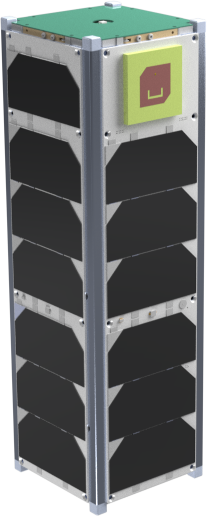
\includegraphics[height=1.3cm]{media/acubesat_small.png}} & \multicolumn{1}{c}{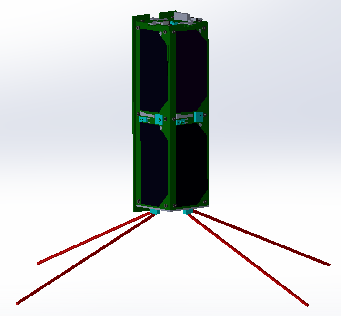
\includegraphics[height=1.3cm]{media/pocketqube.png}} & \multicolumn{1}{c}{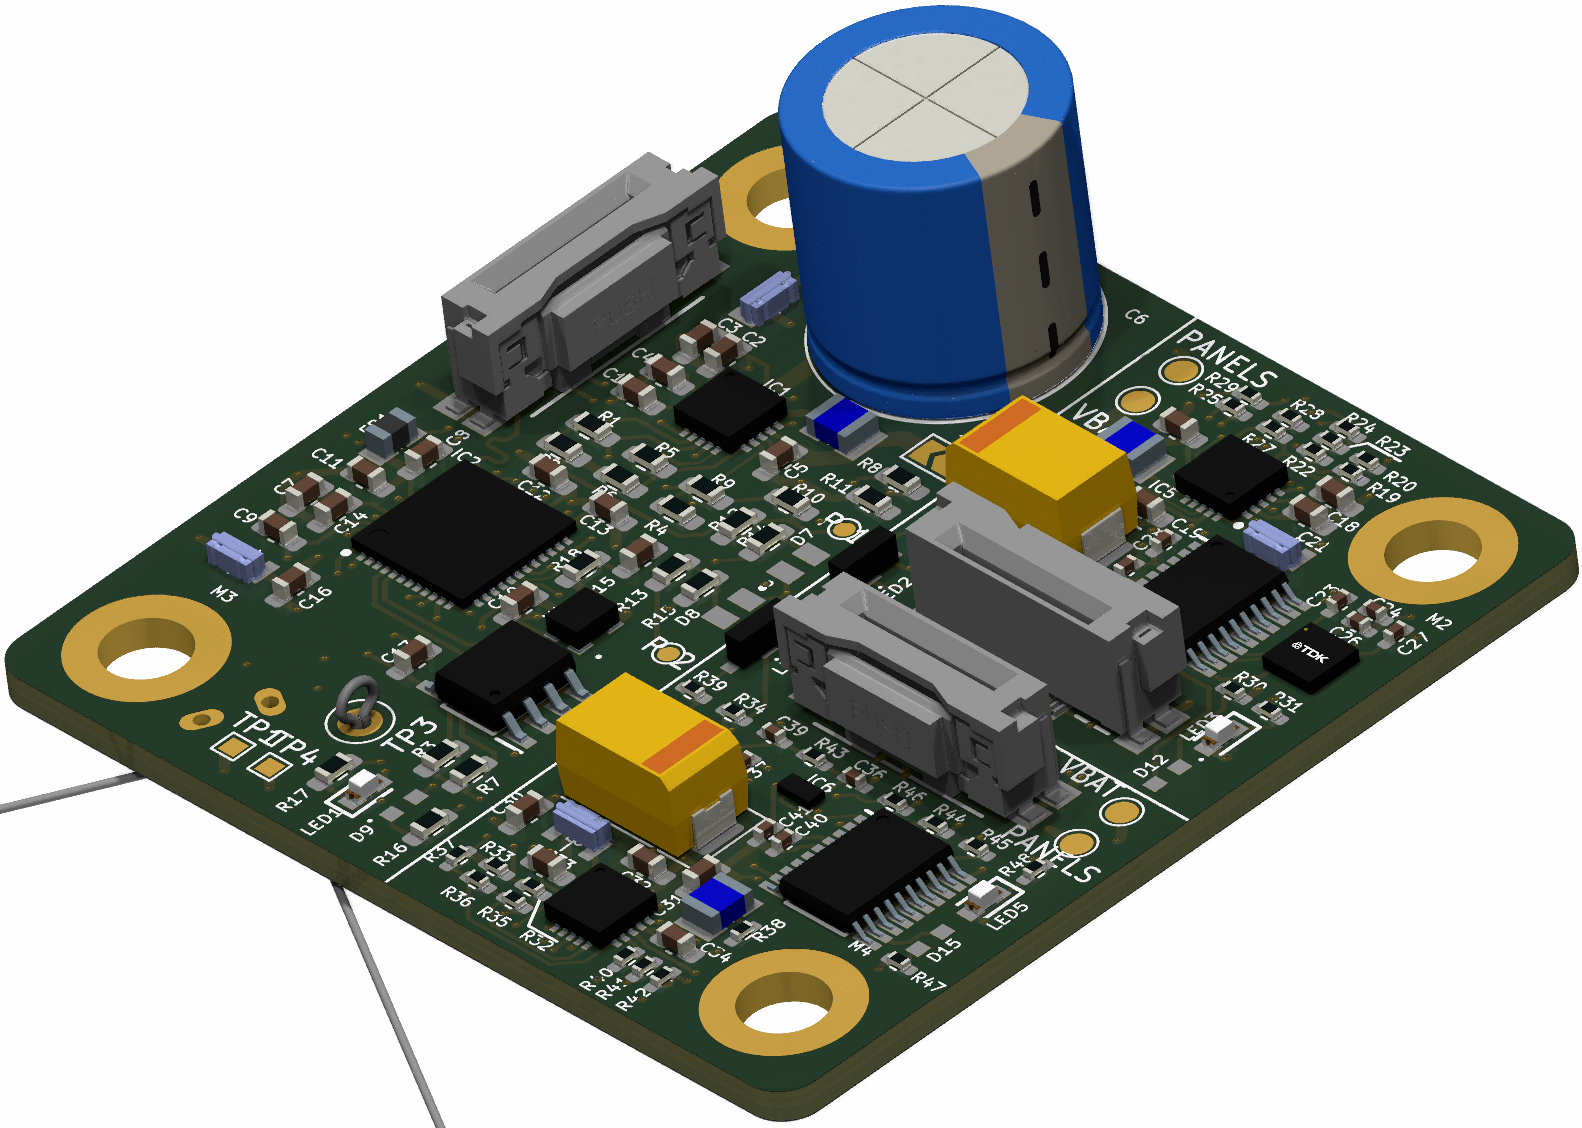
\includegraphics[height=1.3cm]{media/img0913.png}} \\
		\textbf{Scale} & \multicolumn{1}{c}{Nano} & \multicolumn{1}{c}{Pico} & \multicolumn{1}{c}{Femto/Atto} \\
		\cmidrule(lr){2-4}
		\textbf{Mass} & \SIrange{1}{10}{\kg} & \SIrange{0.1}{1}{\kg} & \SIrange{1}{100}{\gram} \\
		\textbf{Fabrication Cost\hspace{-0.3cm}} & \SI{e5}{USD}  & \SI{e4}{USD} & \SI{e3}{USD}  \\
		\textbf{Launch Cost} & \SI{e5}{USD}  & \SI{e4}{USD} & \SI{e3}{USD}  \\
		\textbf{Power} & \SIrange{1}{10}{\watt}  & \SIrange{0.5}{2}{\watt}  & \SIrange{0.1}{0.5}{\watt}  \\ 
		\bottomrule
	\end{tabular}
\end{table}

\subsection{Space Systems Lifecycle Models}
\subsubsection{Spacecraft development approaches}
Space systems development has traditionally followed a top-down, waterfall-like approach \autocite{sheaNASASystemsEngineering2020, ECSS-E-ST-10C}. This waterfall approach on space systems typically follows a set of predefined phases, starting from the mission conceptualisation and technical requirements definition, continuing with the detailed design definition, and finishing with qualification and then flight \autocite{sheaNASASystemsEngineering2020}. This is often modelled as a V-diagram, showing how the system concept influences component design, leading back to system validation in the end \autocite{bundesrepublikdeutschlandVModellXT2006}. Space projects also traditionally follow a \textit{stage-gate} process, where a project is evaluated and its continuation determined at specific points during its lifetime \cite{carsonCanSystemsEngineering2013}.

In addition to this traditional process, incremental or iterative practices are often used \autocite{HEEAGER201822}. \textbf{Incremental} development refers to a method where distinct parts of the design are delivered one at a time; \textbf{iterative} development refers to an approach where the complete system is being refined after each of many cycles --- the goal being that each cycle leads to an improved product, by using the outputs and lessons-learned from the previous cycles \autocite{HEEAGER201822}.
It is also common to use a \textit{hybrid} approach, combining different methods \autocite{carpenterAgileTooFragile2014,garzanitiHybridAgileProduct2020}, for example by using different development lifecycle models in different phases/parts of the project.



\subsubsection{CubeSat development approaches}
\label{sec:approaches}

As CubeSats are the closest to the spacecraft class we are interested in, it is beneficial to focus on the State-of-the-Art of CubeSat development approaches.
Depending of the nature of the project and its team structure, the development lifecycle processes can be categorised as ``single-step'' or ``multi-step'' \autocite{sebok_drivers}.

In \textbf{``Single-step'' approaches}, the typical progression of phases is followed (concept, design, assembly, verification and operations), but with modifications or shortening of each project phase. Usually phases 0, A and B (from conception until preliminary design) are combined into a single Phase AB. In some cases, a demonstration of the mission feasibility using a prototype may be required from Phase AB \autocite{lubian-arenillasNanosatelliteDevelopmentMethodology2019}.

In \textbf{``Multi-step'' approaches}, design, development, and testing may happen concurrently or repeatedly \autocite{lubian-arenillasNanosatelliteDevelopmentMethodology2019,alanaziEngineeringMethodologyStudentDriven2019,sousaCubeSatDevelopmentFramework2021}. For example, it is common to manufacture engineering models or other representations of subsystems, before proceeding to system-wide assembly \autocite{faureLeanSatellitesReliability2017}. It is also common to work in an iterative approach for the entire system, by producing different ``versions'' of a CubeSat \autocite{deckerSystemsengineeringAssessmentMultiple2016,cappaertBuildingDeployingOperating2018}. Iterative development can also happen by working on a reduced version of the entire satellite before assembling; this is often implemented through the ``FlatSat'' approach, where subsystems can be tested long before feature completeness \autocite{nasacubesatlaunchinitiativeCubeSat101Basic2017,MAIVP}. Software, more specifically, can be tested continuously and independently from the rest of the subsystems, leading to quick verification \autocite{kiesbyeHardwareInTheLoopSoftwareInTheLoopTesting2019}. ``Agile'' approaches also fit this category \autocite{labargeCubeSatAgileSystem2014,lubian-arenillasNanosatelliteDevelopmentMethodology2019,garzanitiEffectivenessScrumMethodology2019}.


\subsubsection{Applicability to centimeter-scale spacecraft}


It is generally accepted that single-step and plan-driven approaches are better suited for large projects and teams, which require low risk and predictability \autocite[Sec.~2]{boehmBalancingAgilityDiscipline2004}. These traditional approaches have seen success with large, monolithic missions \autocite{sheaNASASystemsEngineering2020, HEEAGER201822}, especially with safety-critical systems \autocite{kasauliSafetyCriticalSystemsAgile2018}.

However, pico and especially femto and atto-satellites have a number of characteristics (notably low cost and small size) that do not justify the overhead added in each stage of the system design process. More specifically, a traditional approach can add costly overhead in information sharing \autocite{yassineInformationHidingProduct2003}, unnecessary bureaucracy \autocite{boehmBalancingAgilityDiscipline2004}, high inertia \autocite{carsonCanSystemsEngineering2013}, and would not adapt quickly to new technological developments \autocite{sebok_drivers}. In sub-CubeSat developments, prototypes and flight models can be produced with significant ease, as the manufacturing, assembly, integration and verification processes can be performed in smaller time and with fewer resources. As a result, the risk impact of a design error or failure is significantly lower and does not lead to critical consequences, especially since a new physical model can be easily produced.

Furthermore, the ability to verify physical models of the spacecraft during development can allow re-interpreting the design and inspire emergent design solutions, especially in new developments where the solution space is largely uncharted and responsiveness to change may be needed \autocite{dorstCoevolutionEmergenceDesign2019}.


\subsection{Agile}
\label{sec:agilee}

\colorlet{No}{MaterialRed600}
\colorlet{Maybe}{MaterialOrange600}
\colorlet{Yes}{MaterialTeal600}
\def\yes{\textcolor{Yes}{Yes}}
\def\partially{\textcolor{Maybe}{Partially}}
\def\no{\textcolor{No}{No}}
\begin{table*}[t]
	\caption{\emph{Comparison of popular Agile frameworks \autocite{boehmBalancingAgilityDiscipline2004}. \emph{Adaptable to hardware}: Whether the methodology contains elements that can be applicable to a space system, and not just software. \emph{Development lifecycle}: Whether the methodology covers most parts of a spacecraft's lifecycle from design to operation, and not just business practices or concepts. \emph{Small systems}: Whether the methodology can be applied to small, simple systems with small teams}}
	\label{tab:compagile}
	\label{sec:scrum_intro}
	\def\arraystretch{1.1}
	\begin{tabularx}{\linewidth}{@{}L{5cm}@{\hskip 1em}L{1.5cm}L{1.5cm}L{1.3cm}@{\hskip 1em}X@{}}
		\toprule
		& \footnotesize Adaptable to hardware & \footnotesize Development lifecyle & \footnotesize Small systems & Comments \\ \midrule
		\textbf{Kanban} & \yes & \no & \yes &% Does not explicitly address verification/testing
		\\
		\textbf{Scrum} & \yes & \yes & \yes &  \\
		\textbf{Crystal} & \partially & \yes & \yes &  Extensible methodology with different levels; but well-defined only for software \\
		\textbf{Lean Development (LD)} & \yes & \no & \yes & Strategic, risk-driven approach. \autocite{boehmBalancingAgilityDiscipline2004} describes it as \emph{``more a business strategy and project management approach that a development process''} \\
		\textbf{eXtreme Programming (XP)}&\no&\no&\yes &  \\
		\textbf{Dynamic Systems Development Method (DSDM)} & \yes & \yes & \partially & Closer to plan-based ``traditional'' methods, emphasis in management activities.% Some concepts can be applied to small systems.
		\\
		\textbf{Feature-Driven Development (FDD)} & \no & \no & \yes & Mostly focused on software development practices \\ 
		\textbf{Scaled Agile Framework (SAFe)} & \yes & \yes & \no & Built for teams of \(\geq \) 50 people \autocite{heusserTailoringSAFeIt} \\

		%\textbf{Rational Unified Process (RUP)} & ??? & \yes & ??? & ??? \\
		% RUP was a process created by IBM in 2003 that seems to not be supported anymore. There are various notable critics strongly claiming that it has failed, e.g:
		% https://www.quora.com/What-led-to-the-failure-of-the-Rational-Unified-Process-RUP-methodology-Was-it-just-hype-or-were-there-other-factors-involved
		% https://scrumscreener.wordpress.com/2007/02/21/why-rup-failed/
		% https://kenschwaber.wordpress.com/2013/08/06/unsafe-at-any-speed/
		
		\textbf{Disciplined Agile Delivery (DAD)} & \yes & \yes & \no & Covers many other Agile frameworks; resembles a set of guidelines more than a methodology \autocite{ChooseYourWoW} \\

		\textbf{Slice-Based Integration} & \yes & \yes & \yes &  Designed for hardware. Based on Scrum, but product is separated into slices \autocite{iberleAgileGetsPhysical2022a} \\
		\bottomrule
	\end{tabularx}
\end{table*}

``Emergent'' approaches seem to particularly fit sub-CubeSat systems, as they are designed for small systems, with high adaptability to changing requirements and rapid application of lessons learned during development \autocite{sebok_drivers}. These approaches are usually grouped under the term ``Agile'', which originates from the 2021 \emph{Manifesto for Agile Software Development} \autocite{beckAgileManifesto2001}. %, published in 2001, originally aimed towards the field of Software Engineering.


The Agile manifesto includes four values aiming to increase productivity for software development \autocite{beckAgileManifesto2001}.
These values were tailored for systems engineering by \citeauthor{douglassAgileSystemsEngineering2015} \autocite{douglassAgileSystemsEngineering2015}:
\begin{enumerate}[itemsep=0pt]
	\item \emph{Individuals and interactions over processes and tools}
	\item \emph{Verifiably correct specifications over comprehensive documentation}
	\item \emph{Customer collaboration over contract negotiation}
	\item \emph{Responding to change over following a plan}
\end{enumerate}
Agile approaches often follow an iterative cycle \autocite{HEEAGER201822}, each step of which results in a deliverable, working product. 

While Agile originates from Software Engineering and has been observed to improve the effectiveness of engineers \autocite{15thAnnualState,StatusQuoScaled}, it was quickly generalised to systems engineering \autocite{haberfellnerAgileSystemsEngineeringAgileSystems2005}, citing improved engineering efficiency, early Return On Investment, responsiveness to change and increased project control \autocite{douglassAgileSystemsEngineering2015,kohlbacherAgileSoftwareDevelopment2011,darrinAgileManifestoDesign2017}. 

Agile is usually practiced through one or more frameworks, each of which describes a methodology and process for the development of a product.
Different frameworks usually cover different areas of concern \autocite{boehmBalancingAgilityDiscipline2004}. To find one that would be most suitable for sub-CubeSat spacecraft, we are focusing on the systems engineering aspects of product development, including technical management, system description, and system realisation. However, some existing frameworks are built around business strategies, project management processes and concept development \autocite{boehmBalancingAgilityDiscipline2004}, which are outside the scope of this work. Furthermore, as Agile has its roots in software development, many Agile methods are focused on specific development practices for software. To select methods which can provide insights on systems engineering, especially for hardware and space projects, we catalogued their applicability to systems engineeering in \Cref{tab:compagile}.



Practices considered to be Agile have already been considered and used, partially or completely, in various space missions \autocite{carpenterAgileTooFragile2014, dillonFasterBetterCheaperProjectsToo2015, carsonCanSystemsEngineering2013} and especially in CubeSats \autocite{honore-livermoreCubeSatsUniversityUsing2019,berthoudUniversityCubeSatProject2019}. Agile is often used in small teams with limited resources which require a quick \acl{MVP} and do not have significant risks involved \autocite{carsonCanSystemsEngineering2013}.

It is common to use a \textit{hybrid} approach, combining the agile methodology with traditional approaches \autocite{carpenterAgileTooFragile2014,garzanitiHybridAgileProduct2020}. This combination may either involve different product management techniques in different phases/parts of the project, or the modification of an agile method to closer match the traditional V model.


\section{Methodology for sub-CubeSat Spacecraft}
\label{sec:methodology}


In the following sections, we will present our proposed methodology for sub-CubeSat spacecraft, as a synthesis of: \autocite{estefanSurveyModelBasedSystems2008}
\begin{itemize}
	\item A \textbf{process} for the development lifecycle of the project (\Cref{sec:process,fig:process})
	\item A set of \textbf{methods and guidelines} for specific aspects of spacecraft development (\Cref{sec:systems_engineering_aspects,fig:methodology})
	\item A set of example \textbf{tools} to support the methodology (\Cref{sec:tools})
\end{itemize}

The methodology is summarised in \Cref{fig:process,fig:methodology} and is a result of tailoring of Agile frameworks from \Cref{tab:compagile} (\Cref{sec:task_clarification}) and iterations after application to two case-study missions (\Cref{sec:case_studies}).

\subsection{Task Clarification}
\label{sec:task_clarification}

\begin{figure*}[th]
	\centering
	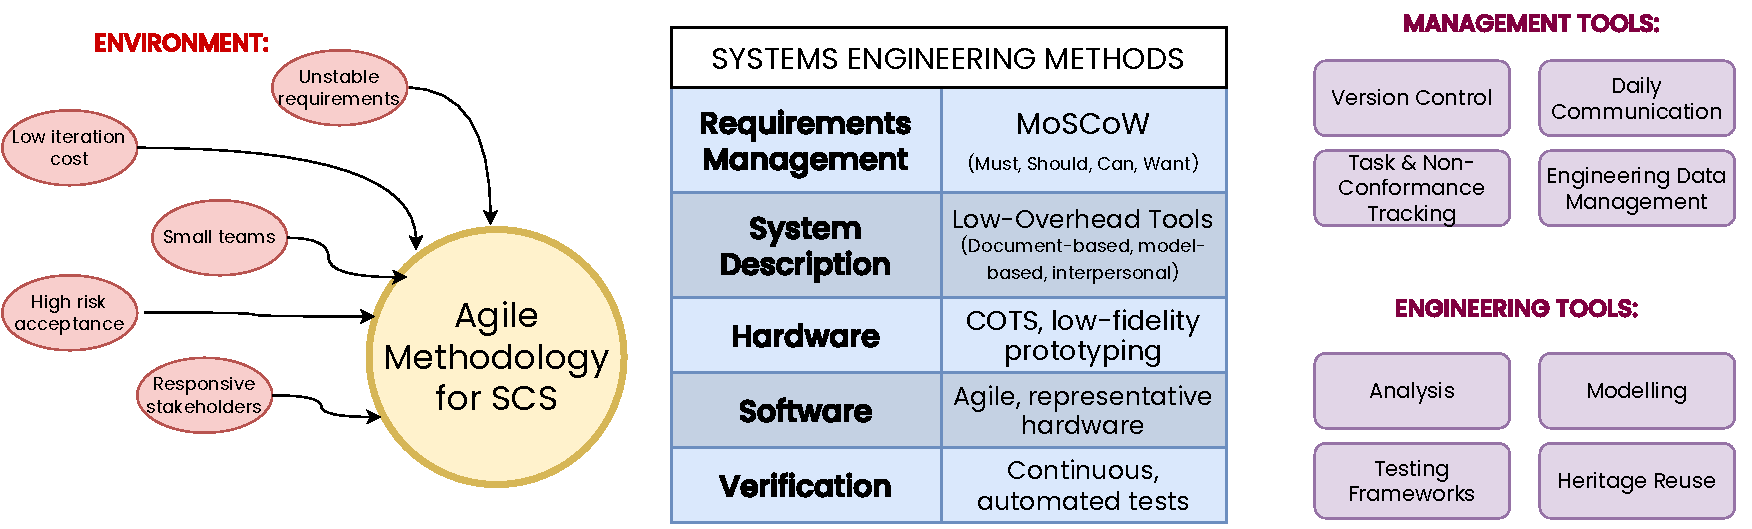
\includegraphics[width=.9\linewidth]{media/AgileMethodology.pdf}
	\caption{Inputs, methods and tools that support the proposed methodology}
	\label{fig:methodology}
%\end{figure*}
%\begin{figure*}[th]
	\centering
	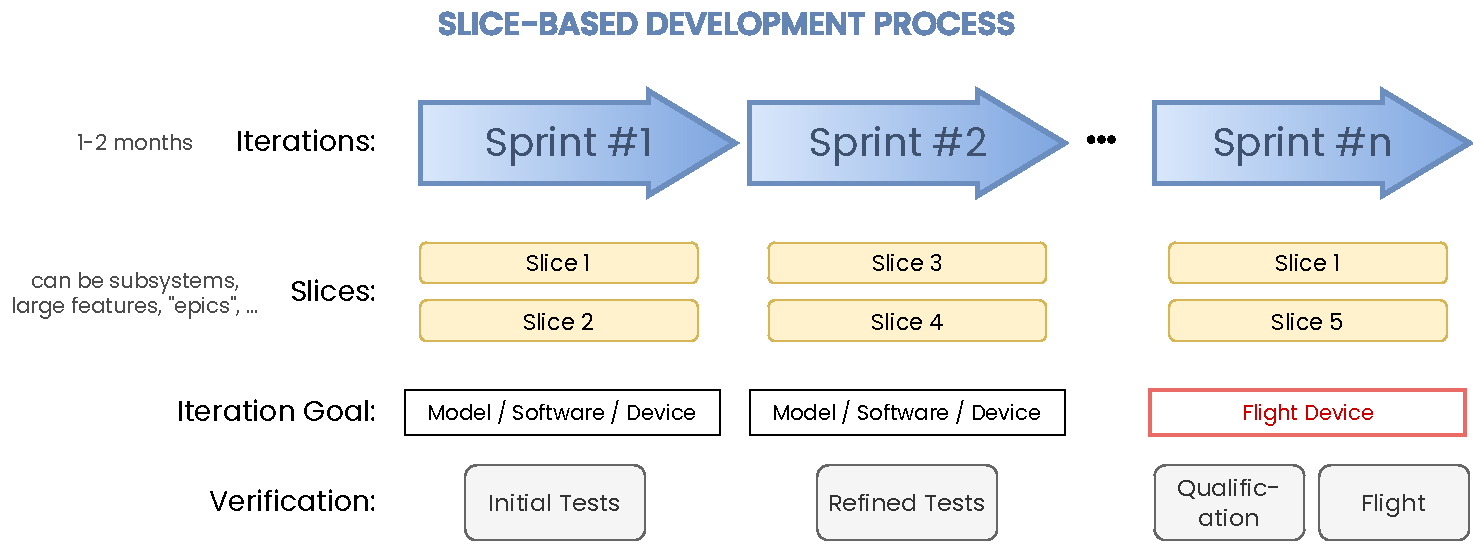
\includegraphics[width=.9\linewidth]{media/AgileProcess.drawio.pdf}
	\caption{The main development lifecycle process of the proposed methodology}
	\label{fig:process}
\end{figure*}


The functions that need to be covered by a development methodology for spacecraft in general can be gathered from different definitions of Systems Engineering \autocite{sheaNASASystemsEngineering2020,ECSS-E-ST-10C}. Therefore, a comprehensive methodology will need to cover the:
\begin{itemize}
	\item Development process \autocite{sebok_drivers}
	\item System Description (design input, modelling, knowledge management, interface management)
	\item System Realisation (implementation, integration, verification)%, operation)
	\item Technical Management (requirements management, risk management, reviews)
\end{itemize}

Even within the sub-CubeSat classes, diverse types and scales of programs exist. These differ in team characteristics, environment and objectives, factors which heavily influence the selection of the methodology \autocite{kalusCriteriaSoftwareProcess2013}. It is therefore difficult to suggest a concrete ``one-size-fits-all'' methodology.

Swartwout \autocite{swartwoutYouSayPicosat2018} proposed a classification that is diverse enough to allow categorizing organizations developing spacecraft based on their organisational status and program scale, into the following \textbf{types}:
\begin{itemize}
	\item \textbf{Hobbyists}: Usually universities, clubs or schools that are developing their first missions. They are often associated with low-cost, lack of standard practices, and high tolerance of risk. Team sizes may range from a few people to many subteams, depending on the project size. Examples include the KickSat project \autocite{manchesterCentimeterScaleSpacecraftDesign2015} or the Libre Space Foundation \autocite{triantafyllopoulouQUBIKProjectReady2020}.
	\item \textbf{SmallSat Developers}: Usually companies or universities with some experience in building satellites, some level of risk acceptance, and a highly iterative approach. Examples include \emph{Alba Orbital} or \emph{Fossa Systems}.
	\item \textbf{Traditional Contractors}: Usually corporations with a long history of developing and flying space missions, with established procedures, facilities, knowledgeable personnel and high performance objectives. Examples include space agencies and large aerospace companies.
	\item \textbf{Constellations}: Developers of small spacecraft constellations are associated with high availability of resources combined with a high tolerance of risk. Examples of constellations in the CubeSat category include \emph{Planet}, \emph{Spire} and \emph{Swarm}.
\end{itemize}


\citeauthor{kalusCriteriaSoftwareProcess2013} \autocite{kalusCriteriaSoftwareProcess2013} has performed a systematic review of criteria for the tailoring of development processes on software, which could also be applied to hardware projects. These can be used to evaluate the applicability of a specific Agile framework to a hardware project. We have therefore catalogued the characteristics of each type of mission, based on these criteria, in \Cref{tab:mission-characteristics}.
We then evaluated each criterion based on \begin{enumerate*}
    \item the definition of each class,
    \item the characteristics of past missions (\Cref{tab:otherdevtime}),
    \item available bibliography \autocite{sweetingModernSmallSatellitesChanging2018,swartwoutYouSayPicosat2018,dillonFasterBetterCheaperProjectsToo2015}, and
    \item personal interactions with the \acs{SCS} community.
\end{enumerate*}

For our analysis, we have ignored the \emph{Constellations} category, as while the mission goals are different, the development process is similar to one of the other three categories, depending on the type of organisation.


\begin{table*}[]
	\caption{Characteristics of different classes of sub-CubeSat programs. Criteria taken from \autocite{kalusCriteriaSoftwareProcess2013}.}
	\label{tab:mission-characteristics}
	\begin{threeparttable}
	\footnotesize
	\begin{tabular}{@{}lL{5cm}L{4cm}L{4cm}@{}}
	\toprule
	& \textbf{Hobbyists} & \textbf{SmallSat Developers} & \textbf{Traditional Contractors} \\ \midrule
	\multicolumn{4}{c}{Team} \\ \midrule
	Size & 10 people or fewer & 20 people or fewer & Large \\
	Distribution & Direct communication between team members & Direct communication between team members & Usually separate contractors \\
	Turnover & Team members have a high turnover rate, limited duration in project & Low or Medium & Low \\
	Previous cooperation & Varies & Varies & High \\
	Good cooperation & Varies & Varies & Varies \\
	Domain knowledge & Usually Low & High & Very High \\
	Tool knowledge & Usually Low & High & Very High \\
	Technology knowledge & Usually Low & High & Very High \\
	Process knowledge & Usually Low & High & Very High \\
	\midrule \multicolumn{4}{c}{Internal Environment} \\ \midrule
	Prototyping & \multicolumn{3}{c}{Low manufacturing cost of satellite would encourage prototyping at all stages} \\
	Clear project proposal & No & Often & Yes \\
	Management availability & High & High & Low \\
	Management support & High & High & Low \\
	Project budget & Low & Medium & High \\
	Project duration & Indefinite & Short\textendash Medium & Long \\
	Project type & Varies & Varies & Varies \\
	Project role & Varies & Varies & Varies \\
	Sub contractors & Rare & Sometimes & Almost always \\
	Financial controlling & High & Low & High \\
	Measurement & Low & Medium & Medium \\
	Technical support & Low & Medium & High \\
	Programming language & N/A & N/A & N/A \\
	\acs{COTS} products
	\tnote{*}
	& Combination of COTS/in-house & Combination of COTS/in-house & Usually \\
	Operating system & N/A & N/A & N/A \\
	Database system & N/A & N/A & N/A \\
	Tool infrastructure & Varies & Varies & Varies \\
	\midrule \multicolumn{4}{c}{External Environment} \\ \midrule
	Legal aspects & Yes & Yes & Yes \\
	Stakeholders & None, one or few (sponsors, launch providers) & Few & Many \\
	Requirements stability & Low & Low & High \\
	Client process & None & None & Alignment with internal/government processes usually required \\
	Client availability & N/A & High & Low \\
	Type of contract & Flexible & Varies & Fixed \\
	User availability & Varies & Varies & Varies \\
	User background & Varies & Varies & Varies \\
	Trainings & Varies & Varies & Varies \\
	\midrule \multicolumn{4}{c}{Objectives} \\ \midrule
	Domain & \multicolumn{3}{c}{Space Engineering} \\
	Complexity & Medium & Medium & High \\
	Degree of innovation & High & Medium & Medium \\
	Legacy system & No & No & No \\
	Conceptual solution & N/A & N/A & N/A \\
	Technical solution & Yes & Yes & Yes \\
	Hardware development & Yes & Yes & Yes \\
	User Interface & N/A & N/A & N/A \\
	System integration test & Required & Required & Required \\
	Neighboring systems & \multicolumn{3}{c}{Deployer/host, and launch vehicle} \\
	Safety \& Security & \multicolumn{3}{c}{Strict requirements from externals (e.g.~launch provider, regulators)} \\
	\bottomrule
	\end{tabular}
	\begin{tablenotes}\footnotesize
		\item[*] Currently, most sub-CubeSat spacecraft are built completely in-house, since there is no significant off-the-shelf subsystem or component availability.
	\end{tablenotes}
	\end{threeparttable}
\end{table*}


Comparing the frameworks of \Cref{tab:compagile} with the characteristics of \Cref{tab:mission-characteristics}, we note the groups of \textbf{Hobbyists} and \textbf{SmallSat Developers} as main groups whose characteristics match those needed for Agile development. We therefore establish the target of our methodology to be academic, non-profit or industrial projects from these groups.

Since the \emph{SmallSat Developers} group in Swartwout's classification is too diverse in itself, we are specifically targetting its lower end: Teams with fewer than 20 developers, rapidly manufacturable designs and centralisation of responsibilities, matching the characteristics in \mbox{\Cref{tab:mission-characteristics}}.

\par

At the same time, we note the key differences between these environments and the assumptions of Agile frameworks, namely:
\begin{itemize}
	\item \textbf{Prototyping}:
	Prototyping software does not require any manufacturing, and verification can be made almost instantly and automatically.
	Prototyping hardware is associated with added cost and time (for production and assembly), manual testing, and limited supply (limited pieces of hardware can be produced and tested at the same time)
	\item \textbf{Complexity}: %While software is inherently complex, space hardware adds an additional degree of complexity, which reduces the benefits added by experience.
	Hardware projects add an additional degree of complexity, further influenced by \acf{COP} \autocite{schmidtAgileDevelopmentConstraints2017}.
	\item \textbf{Safety and security}: Formal verification may be required on items of the system whose failure might be propagated to other systems.
	\item \textbf{Sub-contracting}: Certain tasks within the hardware and systems development context require specialised equipment, skills and facilities to be performed (such as \acsp{IC}, \acs{PCB} manufacturing, analysis software, compliance/environmental testing). These tasks often act as blocking points in an Agile team's work, delaying the production and verification of prototypes, and significantly lengthening the critical path.
	Alternatives such as in-house production capabilities or careful selection of collaborators can be considered.
\end{itemize}


\subsection{Development Process and Prototyping}
\label{sec:process}

Hardware requires significant effort to be implemented and tested compared to software.

Hardware depends on physical components which are often not manufacturable in-house or are managed by different teams. Examples include \acp{IC}, \acp{PCB}, machined parts and more. While Agile encourages consolidation of development efforts and in-house manufacturing, this is not always possible given the complexity of hardware used. %
Manufacturing and procurement of external parts is unpredictable and adds large delays (weeks to months) between completion of a design iteration and delivery.
Additionally, especially in space projects, complete verification needs to include manual analysis and environmental simulations, which cannot be automated and might require travel to other facilities.

Such constraints to those are referred to as ``Challenges'' \autocite{ullman13ChallengesWhen2019} or ``\acl{COP}'' \autocite{schmidtAgileDevelopmentConstraints2017} and are considered roadblocks to adapting Agile in hardware projects \autocite{petersonWhenWorldsCollide2021}.


Early prototyping and having a ``minimum working model'' of the entire system at any time is viewed as one of the key aspects of Agile, and the Scrum framework in particular \autocite{schwaverDefinitiveGuideScrum2020}, since it allows identifying design issues and necessary changes at any stage during the design process.
\citeauthor{doveFundamentalsAgileSystems2014} \autocite{doveFundamentalsAgileSystems2014} and
\citeauthor{bottAnalysisTheoriesSupporting2019} \autocite{bottAnalysisTheoriesSupporting2019} identified Scrum as a favourable framework for hardware projects, citing its relation to complex system science,
while \mbox{\citeauthor{honore-livermoreDigitalEngineeringDevelopment2022}} \mbox{\autocite{honore-livermoreDigitalEngineeringDevelopment2022}} and \mbox{\citeauthor{garzanitiEffectivenessScrumMethodology2019}} \mbox{\autocite{garzanitiEffectivenessScrumMethodology2019}} have already tailored Scrum for application to CubeSat systems or subsystems.%

In principle, the \textbf{small scale of a sub-CubeSat project} allows \textbf{iterating over the entire assembled system} over a short period (a ``sprint'').

Alternatively, depending on the structure of each development team and the complexity of the system, the project can be split into ``\textbf{slices}'' covering distinct functionalities and components \autocite{iberleAgileGetsPhysical2022a}, which can be iterated over in parallel.
For example, four different versions (\emph{iterations}) of a ChipSat or PocketQube might be produced prior to launch, integrated within a feedback loop that allows applying any lessons learned or design changes to the next iterations \autocite{kanavourasAgileSystemsEngineering2022}.

We present this \textbf{slice-based development process} as the base of our development methodology, as shown in \Cref{fig:process}. Each slice can be a different development aspect, such as \emph{software}, \emph{electronics} or \emph{structures}. Alternatively, a slice can be a major subsystem or feature, such as the payload, communications or power. Each iteration should lead to a product that includes as many slices as possible, so that a representative system can be built and verified as a whole. However, each sprint does not need to iterate on all slices at once.

This iteration-heavy approach can help developers identify design issues and adjust the project direction even early in the development process. This is achieved through planned reviews and retrospective meetings after every iteration. The duration of an iteration is usually \textbf{1 to 2 months}, short enough to allow quickly evaluating the results of the design process, but long enough to allow manufacturing and verifying a prototype of the system. This duration should then reflect a ``miniaturised process'' of a typical spacecraft development, as described in \autocite{schwaverDefinitiveGuideScrum2020}:
\begin{itemize}
	\item Sprint Planning / Conceptual Design
	\item Detailed Design, Development, Coding, and/or Execution
	\item Manufacturing, Assembly and Integration
	\item Verification and Validation
	\item Review and Retrospective
\end{itemize}
The exact allocation of time, slices and personnel of each sprint depends on the structure of the team and the project.
This allocation can be done by analysing key factors related to the frequency and responsiveness to change in a project, noted by 
 \mbox{\citeauthor{honore-livermoreAgileSystemsEngineering2021} \autocite{honore-livermoreAgileSystemsEngineering2021}} to be \emph{dynamics} (how the project changes over time and how the team responds), \emph{visibility} (how quickly the team can react to changes), and \emph{variety} (the uniqueness and diversity of possible changes).%

 
\subsection{Methods for sub-CubeSat space systems engineering}
\label{sec:systems_engineering_aspects}

By dividing systems engineering into the functions (\Cref{sec:task_clarification}) and identifying suitable solutions from different Agile frameworks (\Cref{tab:compagile}), we can present a series of targeted methods for sub-CubeSat spacecraft.

\subsubsection{Human Factors}
\label{sec:humans}


Agile methods are often considered to be driven by human factors and depend more on pre-existing knowledge than plan-driven methods \mbox{\autocite[ch.~2]{boehmBalancingAgilityDiscipline2004}}.
As such, personnel selection is critical for such missions.
	
This is especially harder in academic projects, where participating students may not stay in the project for a long time, and lack prior mission experience {\mbox{\autocite{honore-livermoreIntegratingAgileSystems2022}}}.
	Educational projects typically address these issues by maintaining a core coordinating team of experienced and dedicated engineers, accountable for administrative and technical aspects, who are also responsible to maintain knowledge transfer within the team across different flight projects {\autocite{berthoudUniversityCubeSatProject2019}}. For teams with fewer experienced members, access should be provided, if possible, to domain experts who can offer high-level feedback, especially during the retrospective phases of each iteration.

Projects should also experiment to identify the ideal communication and collaboration model based on their environment. A common working space, combined with transparent information sharing and frequent workshop/training sessions can lead towards that goal, especially for smaller teams {\autocite{honore-livermoreCubeSatsUniversityUsing2019}}.%

Frequent informal reviews are also recommended to be performed at a high level before manufacturing.
	Research in Software Engineering suggests that reviews by at least one person with a carefully selected frequency can significantly aid in the early detection of defects \autocite{kemererImpactDesignCode2009}.
	We therefore suggest that each significant discipline is represented by at least two members in a development team, who can review each other's design results at every iteration.%

Framework and tool selection further play a critical role in team communication. Instead of compartmentalisation, we encourage all information to be publicly shared but well organised, so that all participants can have a direct view of the project and subsystem status.

\subsubsection{Requirements Management}
\label{sec:methodology_requirements}

Space engineering reference literature advocates for the use of requirements in all development phases of a project \autocite{sheaNASASystemsEngineering2020,ECSS-E-ST-10C}. Strictly defined requirements specified in the early project stages are used to define its verification methods and success criteria \autocite{ECSS-E-ST-10C}. However, physical constraints combined with the lack of standardisation in the field lead to many unavoidable requirements changes during development.

The \acs{DSDM} methodology advocates the prioritisation of requirements using \acf{MOSCOW} prioritisation, where ``traditional'' requirements would be classified as ``must-haves'', and optional features are classified as such \autocite{agilebusinessconsortiumAgilePMHandbookV22014}. Requirements can also be considered as ``user stories'' or features to be implemented in a project. The developers also have the possibility of moving a requirement to a future iteration, classifying it as a ``won't have this time'' requirement. This follows the basic Agile principles \autocite{beckAgileManifesto2001}, based on which project requirements are not set in stone, but can be modified with customer participation.

This approach goes \emph{against} the idea that ``there is no justification for designing something one bit better than the requirements dictate'' \autocite{akinAkinLawsSpacecraft}, noting that optional requirements can provide value to a customer or organisation even when they are not absolutely necessary for the completion of a project.


\subsubsection{Documentation and System Description}
\label{sec:documentation}

\citeauthor{sanchez-rosadoAssessingDocumentationDevelopment2009}
\autocite{sanchez-rosadoAssessingDocumentationDevelopment2009} estimated that 12\% to 35\% of a software project's development time is spent on documentation. To optimise this effort, an Agile hardware project should consider the following aspects:
 \begin{itemize}
	\item \textbf{Completeness}: The documentation should be able to describe the system as accurately as needed, especially on any external interfaces.
	\item \textbf{Efficiency}: Documentation should require a minimal amount of effort and time from the developers to produce and maintain, especially in small teams.
	\item \textbf{Flexibility}: Even small spacecraft are complex systems-of-systems that contain different types of interfaces.
	Prose is inherently more flexible in describing such complex relationships compared to simplified models.
	\item \textbf{Accessibility}: Apart from being easy to write, documentation should be easy to read; engineers should spend the minimum amount of time and actions to access a description or parameter.
	\item \textbf{Maintainability}: Documentation should not be kept outdated, and incentives should be given to keep it maintained and updated at regular intervals. Automated tools could be significantly useful in this case.
\end{itemize}

We note that even when documentation is available, teams (especially with less experience or in fast-paced environments)
	may not use it consistently, influenced by impractical documentation tools or lack of encouragement from the systems engineers \mbox{\autocite{honore-livermoreAgileSystemsEngineering2021}}.
	The documentation process therefore also depends on regular maintenance and tool selection. \mbox{\Cref{tab:documentation}} compares four types of documentation-producing tools (see \mbox{\Cref{sec:tools}}).%


\def\highbad{\textcolor{No}{High}}
\def\highgood{\textcolor{Yes}{High}}
\def\lowbad{\textcolor{No}{Low}}
\def\lowgood{\textcolor{Yes}{Low}}
\def\depends{\textcolor{Maybe}{Varies}}
\begin{table}[h]
	\centering
	\caption{Comparison of documentation methods}
	\label{tab:documentation}
	\begin{tabular}{@{}lllll@{}}
			\toprule
	 & \multicolumn{2}{c}{Document-based} & \multicolumn{2}{c}{Model-based} \\ \cmidrule(r){2-3} \cmidrule(r){4-5}
	 & \textbf{Informal} & \textbf{Formal} & \textbf{Informal} & \textbf{Formal} \\ \midrule
	\textbf{Completeness} & \lowbad  & \highgood  & \depends  & \highgood  \\
	\textbf{Efficiency} & \highgood & \lowbad  & \highgood & \lowbad \\
	\textbf{Flexibility} & \highgood & \highgood  & \lowbad  & \highgood  \\
	\textbf{Accessibility} & \highgood & \lowbad  & \depends  & \lowbad  \\
	\textbf{Maintainability} &  \highgood & \lowbad  & \depends & \lowbad \\
	\bottomrule
	\end{tabular}
\end{table}

Apart from description-based documentation methods, Agile frameworks such as \ac{DSDM} \autocite{agilebusinessconsortiumAgilePMHandbookV22014} advocate for the use of alternative forms of communication, such as:
\begin{itemize}
	\item Team Boards (graphical representation of project information and status) \autocite{agilebusinessconsortiumAgilePMHandbookV22014}
	\item Training sessions, tutorials and workshops
	\item Self-documenting code \autocite{amblerStrategiesAgileSoftware2008}
	\item Executable specifications \autocite{amblerStrategiesAgileSoftware2008}
	\item Large Language Model (LLM)---based documentation
\end{itemize}

The process for interface management with other entities (e.g.~launcher) might be different, and usually stricter than the internal team documentation, due to the former's higher criticality.

\subsubsection{Implementation and Integration}
\label{sec:methodology_implementation}

The definition and implementation of the design solution for a sub-CubeSat satellite is split into \emph{hardware} (including electronics and mechanical parts) and \emph{software}.

For hardware, considering the lower cost and need for simplicity, we can consider that:
\begin{itemize}
	\item Standard, off-the-shelf parts and processes are preferred to reduce lead time and increase repeatability. Radiation-tolerant parts can be avoided, circuit boards should follow standard formats, and manufacturing tolerances should not be strict.
	\item Prototyping can be made at different levels of representativeness, and as early as possible. Examples of low-fidelity parts include 3D-printed parts, Breadboard Models, Development Models, or Mock devices.
	\item Depending on the device, modularity might need to be carefully considered. Devices with non-standard shapes (e.g.~ChipSats) or limited space might be impeded by the overhead added by modularity.
\end{itemize}

Regarding software, while the typical aspects of Agile software development are applicable to space systems \autocite{boehmBalancingAgilityDiscipline2004}, some aspects specific to sub-CubeSat spacecraft are:
\begin{itemize}
	\item Ideally, software will be developed on representative hardware, such that any constraints or issues caused by hardware differences are identified as early as possible. In the absence of representative hardware, simulators or mock-ups can be used, as long as they do not require disproportionate effort to implement. Remote or concurrent access to hardware is highly desirable as well.
	\item Based on the project, different programming languages or techniques can be used, with the aim of increasing reliability without sacrificing development speed. Examples include static analysis, automated testing/fuzzing, Design by Contract (DbC), Domain-Specific Languages (DSLs), or automated code generation.
\end{itemize}

Finally, for both aspects, technology and code reuse is highly encouraged \autocite{heinHeritageTechnologiesSpace2016}.

\subsubsection{Interfaces}
\label{sec:methodology_interfaces}

\emph{External interfaces} with the launch provider or other entities may require components not directly available to the development team.
As such, they may not be available for immediate experimentation and testing within a few sprint, and require specific attention during development 
	\autocite[95]{honore-livermoreIntegratingAgileSystems2022}.

Such interfaces and interface requirements can be categorised into:
\begin{itemize}
	\item Mechanical (e.g allowable envelope, fasteners, load limits)
	\item Electrical (e.g interconnects, voltage/power limits, dep\-lo\-yment swit\-ches)
	\item Software (e.g protocols, data rates, packet throughput)
\end{itemize}


As interface compliance is a ``must-have'' requirement for all missions, interfaces should be implemented early in the design and documented in greater detail than the rest of the system.
Depending on the launch opportunity selected, hosts may agree on a specific interface with their guests, share detailed documentation, or provide ``mock'' interface simulators to them.
Developers should validate interfaces as early as possible, and attempt to integrate prototype implementations with the host's systems (``hardware-in-the-loop'' testing \autocite{honore-livermoreDigitalEngineeringDevelopment2022}). This will allow them to follow the need for system-level verification at every iteration of our process.
They should also be cautious of revisions, especially when the flight heritage of their host is limited.

If possible, developers should be physically present to verify the final hand-off or integration before launch, and allow for a few days to correct small deviations if needed.
	
In some cases, the criticality of such interfaces might be high enough to require proof that no system external to the satellite might be negatively impacted.
Metrics such as the ECSS severity scale \autocite{ECSS-Q-ST-30-02C} can be used to classify this impact, ranging from \emph{negligible} to \emph{catastrophic} (such as loss of launcher or major injury) effects.
For example, an {\ac{ISS}} launch may have specific limits on electrical system configuration, deployment switches and battery cell heritage.
Interfaces with \emph{catastrophic} failure modes should be verified formally and independently from the rest of the system, as risk cannot be tolerated in this case.%


\subsubsection{Verification}
\label{sec:methodology_verification}

Verification is both an integral part of every sprint/iteration during development, and also typically formally requested by launch providers.
Verification is usually done through \emph{review of design}, \emph{analysis} or \emph{testing}/\emph{inspection} \autocite{ECSS-E-ST-10C}. By default, Agile methods place significant focus on testing, as it can be done early and continuously on representative units. However, each organisation can choose to prioritise other methods based on the context, the acceptable risk, and a cost analysis.


For system-level tests, a large part of the typical space test suite \autocite{ECSS-E-ST-10-03C}  is also applicable to sub-CubeSat spacecraft, including Functional Tests (full tests, ``day-in-life'' tests, or failure recovery tests), Integration Tests with neighbouring systems (e.g.~ground station) and Environmental Tests.

In the Agile context, many of the above test can be performed at low costs even during the first iterations on the complete system. \acf{CI} processes can include automated testing procedures that cover software and hardware \autocite{carsonCanSystemsEngineering2013}.

While most satellite manufacturers have the capability to perform electrical and functional testing in-house, environmental testing (vibration, thermal-vacuum or \acs{EMC}) often requires external contractors and/or complicated logistics procedures to complete. In some cases, \textbf{launching a prototype} as part of the verification process can be easier and more effective than performing more accurate testing or analysis. This is, for example, the approach taken by the \emph{SMOG-1} PocketQube team, who launched \emph{SMOG-P} as an early prototype \autocite{SMOG14thHungarian2021}.

Structural and thermal analysis can also be performed as a design driver on a per-project basis. For extremely low complexity projects, such as ones consisting of single \acs{PCB}, mechanical and thermal characteristics may be empirically known by the development team. As such, no analysis or calculations will be required. This might be in contrast to a PocketQube with complex mechanical/thermal interfaces, which may need to be analysed beforehand.
	
The choice on the ideal number of tests and analyses ultimately depends on the logistical situation of the project team.
	For example, depending on available personnel, facilities, administrative support, and required results, an additional test may be easier than setting up an analysis.


\begin{table*}[bth]
	\caption{Indicative systems engineering tools to support agile sub-CubeSat development}
	\label{tab:indicative_tools}
	\begin{tabularx}{\linewidth}{@{}llX@{}}
	\toprule
	\multicolumn{2}{l}{Task} & Example Tools \\ \midrule
	Project Management and Planning &  & Jira, OpenProject, Plane, Wrike, Trello \\
	Internal Communication & & Slack, Mattermost, Zulip, Discord, Microsoft Teams, Zoom \\
	\multirow{4}{*}{Knowledge Management} & Document-based informal & MkDocs, Sphinx, Doxygen, Excalidraw, \textit{Wiki software} \\
	 & Document-based formal & Microsoft Office, LibreOffice, LaTeX \\
	 & Model-based informal & CDP4-COMET, Valispace \\
	 & Model-based formal & SysML, Capella, Papyrus, Cameo Systems Modeler, Enterprise Architect \\
	Asset Management & & Inventree, ERPNext \\
	Artifact Management & Software and hardware & Github, GitLab \\
	Requirements Management &  & Jira, Notion \\
	Test and Defect Management &  & Jira, Notion \\
	Verification &  & LabView, Selenium, Python Robot Framework \\
	\multirow{2}{*}{Implementation} & Hardware & \textit{3D printers, multiphysics simulators} \\
	 & Software & \textit{Design by Contract, Code Generation, In-orbit scripting} \\
	 \bottomrule
	\end{tabularx}
\end{table*}

\subsection{Tools}
\label{sec:tools}

A variety of tools are available to support Project Management and Systems Engineering activities of Agile projects. 
While the selection of a tool depends significantly of the environment in every space system organisation, we note that aspects such as employee familiarity with tools, need for training, available features and usability can have a significant impact on the administrative and time overhead in a project \autocite{honore-livermoreDigitalEngineeringDevelopment2022}.
Indicative tools usable within the context of sub-CubeSat spacecraft are listed in \Cref{tab:indicative_tools}.

\begin{table}[h]
	\centering
	\caption{Project Management details for both projects}
	\label{tab:case_pm}
	\begin{tabularx}{\linewidth}{@{}lXX@{}}
		\toprule
		& AI4Space & ChipSat-1 \\ \midrule
		Team size & 4 (\textasciitilde 40\% allocation) & 7 (\textasciitilde 40\% allocation) \\
		Type & Interfaced Payload & Mounted payload \\
		Duration & 14 months & 12 months \\ % concept to delivery
		Fabr. cost / sprint & 1000€  & 3000€ \\ % based on budgets
		% difficult to get an accurate number per iteration, since we made orders in bulk
		% single-board cost ranges from 300-1500€ for both projects
		Tests done & Functional & Functional, vibration, thermal \\
		\bottomrule
	\end{tabularx}
\end{table}

\begin{table}[h]
	\centering
	\caption{Results for both projects}
	\label{tab:case_result}
	\begin{tabular}{@{}lll@{}}
		\toprule
		& AI4Space & ChipSat-1 \\ \midrule
		Working Iterations & 2 & 4 \\
		Non-Conformances (total) & 11 & 20 \\
		Non-Conformances (final) & 5 & 6 \\
		Status & Operational & Pending launch \\%Launch cancelled} \\
		\bottomrule
	\end{tabular}
\end{table}



\begin{figure*}[h]
	\centering
	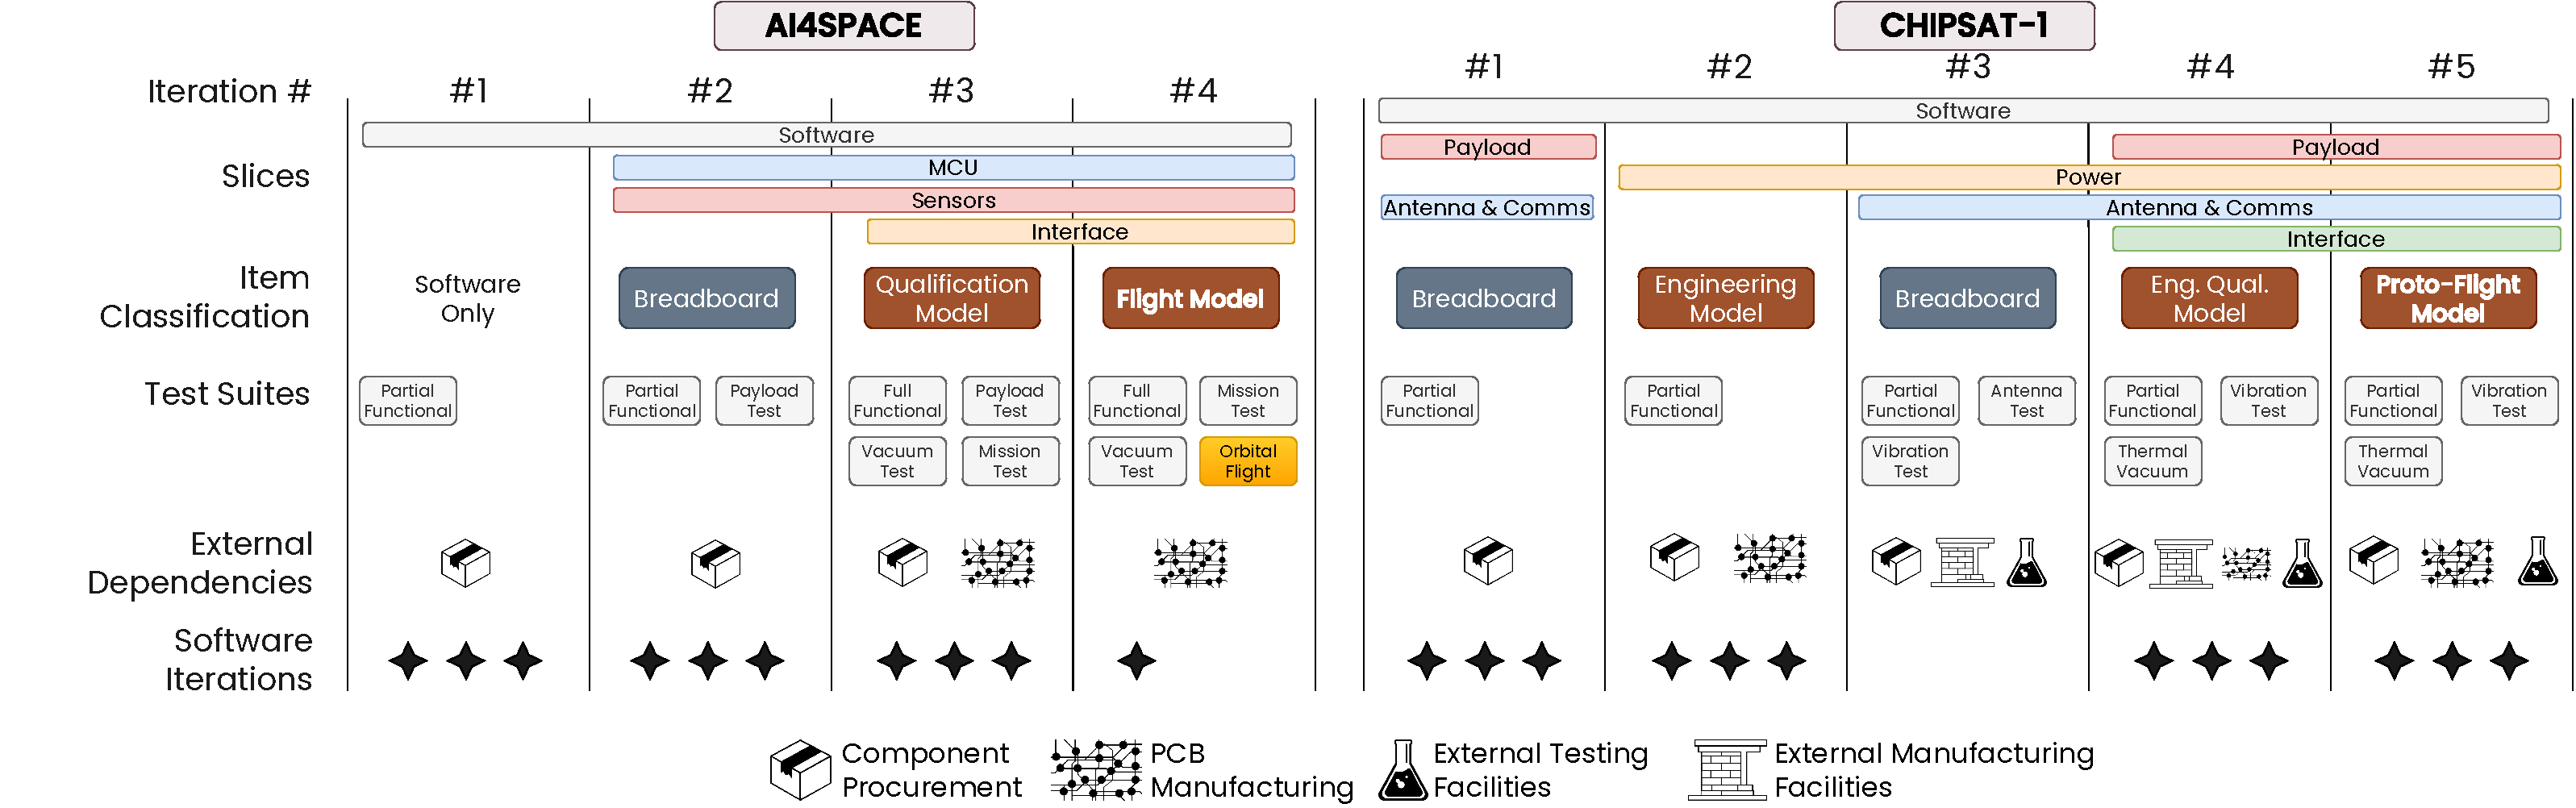
\includegraphics[width=\textwidth]{media/AllProjectSlices.drawio.pdf}
	\caption{AI4Space and ChipSat-1 iterations}
	\label{fig:project1scrum}
	\label{fig:project2scrum}
	\label{fig:scrums}
\end{figure*}


\section{Case Studies}
\label{sec:case_studies}

In this section, we will provide details on the Case Studies
used for the experimental validation and fine-tuning of the approach. The projects that were used were the following:
\begin{itemize}
	\item \textbf{AI4Space}: A payload board, consisting of a single \qtyproduct[product-units = single]{10 x 10}{\centi\metre} \ac{PCB}. The board was designed to test the use of edge \acl{AI} in thermal anomaly detection \autocite{thoemelLeanDemonstrationBoard2024}.%\autocite{thoemelAI4SpaceSnTLaunches}.
	\item \textbf{ChipSat-1}: An independently-operating ChipSat (\qtyproduct[product-units = single]{5 x 5}{\centi\metre} \ac{PCB}), mounted on another satellite. This femto-satellite is intended as a technology demonstration mission, emulating a fractionated system with visible light communications \autocite{borgueDevelopingDistributedFractionated2022a}. %REDACTED
\end{itemize}

Both missions were developed within one year in the Interdisciplinary Centre of Security, Reliability and Trust (SnT) in the University of Luxembourg,
with teams composed by co-located students and researchers.


An Agile approach was followed for both projects, converging towards the methodology described in \Cref{sec:methodology}. We followed the principle of \text{action research}, by establishing a plan of action for an iteration, implementing it, and using lessons-learned as feedback to improve the methodology for the next iteration \autocite{mcniffActionResearchPrinciples2003}. 


Key values about the projects are shown in \Cref{tab:case_pm,tab:case_result}.
Despite sharing a common goal (technology demonstration) and shape, both projects present major differences in terms of interfaces and development focus. AI4Space is a software-heavy project, where the power, communication and interfaces were already provided by the host. ChipSat-1 was a hardware-heavy project, where the physical interfaces and main spacecraft functions had to be implemented from scratch, while the software had limited responsibilities. The different technical context of the missions, combined with them being managed and realised by different groups, qualify them as two distinct case studies.

The development timelines of both projects are shown in \Cref{fig:scrums}, following the slice-based approach presented in \Cref{sec:process}.
In both projects, extensive prototyping was done from the first weeks of development, including procurement of components and construction of representative systems. This proved to be a driver for many early design decisions.
The timelines show how each project is separated into different iterations time-wise, during which different ``slices'' of the hardware are iterated upon. After every iteration, a selection of system tests was performed. Software development was not directly tied to the hardware, and thus happened in smaller iterations. 




AI4Space was successfully launched on its host satellite in 2023, and is communicating with the host and performing its main mission.
ChipSat-1 is due to be launched in 2024.


\subsection[Specific Lessons Learned]{Specific Lessons Learned}


\subsubsection{Hardware and Procurement}

As both projects mainly consisted of a single circuit board, {\acf{PCB}} designs were at the core of development.

The PCB of AI4Space was designed in a single iteration by one team member, and was reviewed by another. The review identified all defects except two minor ones. In ChipSat-1, the lack of PCB reviews led to the need for three iterations in order to permanently resolve the identified defects.

%ChipSat-1 also required a mechanical support structure, which had to be procured from an external \acs{CNC} manufacturer. %TODO

The use of in-house developed \acsp{PCB} also introduces an important question: Whether component assembly should be performed in-house or by an external provider.
%While the exact answer will again depend on the project and its relations to its suppliers, 
Using an external provider can lead to communication errors, administrative overhead, lack of process visibility and unpredictable, long lead times. On the other hand, in-house assembly may suffer from lower quality and a need to maintain equipment and train personnel to perform flight-quality component soldering. %However, the need for fast reworks mentioned above will often necessitate in-house operations.
%The discovery of defects on both projects also often necessitated resolving them in-house
However, in-house assembly was often needed in our projects to solve defects, in order to not block the development path by weeks, waiting for the next iterations of the boards. 

%The main obstacles in the critical path were interfaces with external providers and collaborators. The typical procurement times of \acp{PCB} and components were significant and had to be planned around. Any unexpected delays also significantly influenced progress towards the iteration goal. While preparation for such cases might be possible in some contexts, Agile frameworks usually suggest maintaining direct communications with external collaborators, to the extent possible.

As such, our recommendation is to perform in-house assembly for the first iterations, and use external suppliers for the ready-for-flight ones. This allows the earlier, high-risk steps to be dealt with in a way that suits the Agile process, while freeing developer time and increasing reliability for the final flight model. In this case, more specific instructions and photos of the previous assemblies can also be sent to the external supplier to ensure there are no communication errors.

Sub-CubeSat teams should anyway acquire access to in-house equipment and expertise to detect and resolve defects, without needing to rely on external deliveries. This equipment can include, for example, soldering rework stations, 3D printers, thermal chambers or \acs{CNC} mills \autocite{honore-livermoreDigitalEngineeringDevelopment2022}.

These recommendations also apply to mechanical components, and especially environmental testing fixtures, which need to be procured well before (usually \textgreater1 month) a test campaign.
We also recommend maintaining a sufficient redundant stock of spare components, especially mission-critical ones during periods of chip shortage.


\subsubsection{Software Design}
ChipSat-1 was developed in C++ under a \acf{RTOS}, while AI4Space executed Python code under Linux. While Linux is more computation and energy-intensive, its use provided much more development flexibility compared to an \acs{RTOS}. Critical functions such as software patching, error handling and logging need little to no effort to implement under Linux.
 
While using a full Linux distribution may be prohibitive in a low resource system such as a ChipSat, we strongly encourage developers to take ease of development into account when planning their software stack. As an example, the PyCubed-Mini project \autocite{hollidayPyCubedOpenSourceRadiationTested2019} allows full control of a PocketQube's microcontroller strictly using Python.


AI4Space also saw success in combining documentation and implementation, by using a model-based description of all Telemetry and Telecommands in software. A simple \ac{CI} script would then generate human-readable documentation out of this description.

\subsubsection{Documentation}
No extensive documentation was written for both projects (except for host interfaces), as instead we relied on more
interpersonal means of communication.

This was sufficient for most of the day-to-day engineering work, but required additional effort and time when onboarding new members or communicating project status and details with external entities.

While AI4Space was a one-shot project, ChipSat-1's design had to be reused internally. The lack of extensive documentation for the latter led to six weeks of mentoring required during the onboarding of the next project's development team.


In our experience, we found the following aspects of technical documentation to be the most useful and referred to:
\begin{enumerate}
\item Mission objectives, goals and constraints
\item High-level parameters (e.g.~mass, size, trajectory)
\item Iteration timeline and current status
\item System-level budgets (e.g.~mass, volume, power, data)
\item Clarification of high-level design choices
\item High-level schematics (e.g.~top-level block diagram, hardware interface diagram, software interface diagram)
\item Usage/reproduction instructions of hardware and software
\end{enumerate}

We therefore consider informal and document-based documentation (\Cref{sec:documentation}) containing the above as a balanced option for \acs{SCS} projects. This approach allows easy access to a centralised source of information, letting developers elaborate personally on low-level details if and when needed.


\subsubsection{Verification}
Functional verification was performed at system level during each system iteration of the projects, following \Cref{fig:scrums}.

ChipSat-1 was functionally verified manually at software level. In AI4Space, we also established an automated testing procedure based on procedural blueprints. There, tests were executed ``in-the-loop'', using a hardware interface simulator.

No vibration or thermal analysis was performed for either project, as they both consisted of a single PCB with well known mechanical and thermal characteristics, for which empirical knowledge and design reviews were considered adequate.
Both projects successfully passed qualification or acceptance campaigns, performed individually or as part of their host.

Specifically for the ChipSat-1 project, we performed an ad-hoc vibration test during Iteration \#3 (\mbox{\Cref{fig:scrums}}) to experimentally measure the dynamic envelope of the antenna elements. The selection of a test instead of analysis was influenced by the uncertainty of a potential simulation and by a lack of structural analysis engineers in our team.

\subsubsection{Operations}

AI4Space has been operational in orbit, leading to early results from in-orbit validation. Two major non-conformances were discovered during flight. Both revolved around the host-to-guest data interface:
% Packet types:
% TC/Data: Executed by guest, but no data is returned
% TC/ RFD: Host only supports empty RFD, but guest expects data
% TM/ ACK: Supported
\begin{enumerate}
	\item The host transmitted telecommand packets at a much higher throughput than AI4Space could respond to, leading to many of them being discarded.
	\item The host interface specified that AI4Space could send telemetry only after receiving a ``Request For Data'' (\acs{RFD}) telecommand from the host. We expected that \acs{RFD} commands could include a payload of a few bytes. This payload would then specify the kind of telemetry that AI4Space would respond with. However, the actual implementation on the host spacecraft did not include a payload in RFD commands. As such, AI4Space returned only an error on every \acs{RFD} received, with no other way of downlinking telemetry.
\end{enumerate} 

The above non-conformances resulted from a wrong understanding of the host packet protocol, despite successful tests with the host interface simulator. Their combination essentially led to no telemetry being received on the ground from AI4Space.

Despite this, a series of Python patches was created and uploaded, through Linux terminal commands, re-implementing the relevant parts of the protocol and allowing us to perform the experiment as planned, albeit with lower data throughput. The flexibility of Linux as a platform allowed storing these patches as separate files that were executed manually after every boot. We could therefore test their function without risking dangerous and permanent modifications to the flight software. Each patch was validated on the Qualification Model on ground before upload.

After implementing the patches, AI4Space operated consistently in orbit and started producing experimental images.
While we already had semi-automated operations procedures in place,
they could not be used as-is, due to the previously mentioned non-conformances and small differences in the operational conditions of our host (such as experiment duration, experiment count and maximum number of uploadable commands).
Therefore, we initially followed a manual procedure to downlink, store and analyse generated data, and started progressively moving towards a more automated software framework.

While it may have been possible to account for these potential deviations before launch, this would imply considerable effort from our developers.
In our case, we saw success by keeping at least some core developers in the team after launch, so that they can respond quickly to make any necessary modifications.



\subsubsection{Project Management}

The main driver behind project management efforts for both spacecraft was an environment of quickly changing requirements and constraints.

Both projects were within the first payloads integrated by their hosts. Due to this, combined with their form factor, the interfaces between guest and host either did not follow a predefined standard, or had to be revised and clarified frequently. 

For the ChipSat-1 project,
we also had to iterate on requirements such as allowable envelope, antenna location, electrical inhibits and materials.
Unexpected verification and compliance changes from the host's launch provider, such as an increase in the random vibration testing levels, were also passed down to our team. This resulted in a constant need of updates to our flight hardware, something hindered by a 1-month lead time for external assembly. Both projects also went through frequent personnel changes, adding further unexpected delays.


For the AI4Space project, we planned a \emph{Design--Breadboard Model--Qualification Model--Flight Model} path (\Cref{fig:project1scrum}), with only a single \ac{PCB} procurement cycle. In hindsight, it would be preferable to replace the early \emph{Design} and \emph{Breadboard} phases with prototypes of the actual \ac{PCB}, as done in ChipSat-1. This would make early results more representative, reduce time needed to create a breadboard model, and provide more opportunity to revise the design if needed later. While potential technical improvements could be identified to resolve defects and increase performance, the plan for a single \ac{PCB} revision prevented them from coming into fruition.



The critical path of both projects was dominated by procurement times of both electronics and \acsp{PCB}, particularly due to slow administrative procedures in our University.

Project Management artifacts, such as Gantt charts, Requirements Specifications, Non-Conformance Reports and Work Packages were elaborated for both projects, and were consulted on a semi-regular basis.
However, due to them being spread over different files, navigation was impractical, any changes had to be manually communicated to project members, and they were additionally not kept up-to-date consistently.
This led to inconsistent data across different sources, reduced visibility of the project status to its participants, less control over followed deadlines and iteration timing, and reduced the sense of urgency for remaining tasks.

We expect that the use of dedicated, low-overhead tools for project management and team communication would have resolved most of the above issues, outweighing the additional cost and effort required for their integration.


\subsection[Discussion]{Discussion}

\hspace{0pt}\par
Both missions that we presented as case studies managed to be completed by a small team of developers within approximately a year, reaching the construction of a flight model and their functional goals (and in the case of AI4Space, a successful in-orbit demonstration), and demonstrating the applicability of Agile methods to our environment.

We noted these particular aspects of our methodology as having the most positive impact on the projects: 

\begin{itemize}
	\item \textbf{Early prototyping} of the entire systems (\Cref{sec:process}) was incredibly beneficial; Despite the additional effort and need for revisions, the experiences gained by having functional prototypes removed the need for estimations and guesswork, especially during the early stages of the project.
	\item Early iterations on the actual \textbf{flight design} can prove more beneficial and time-saving than low-fidelity representations such as breadboard models (\Cref{sec:process}).
	\item Even if some sprints only iterated on some slices of the project, we had to \textbf{verify the entire system} at the end of the sprint (\Cref{sec:methodology_verification}). This prevented any interface and compatibility issues between subsystems and increased confidence in the function of the system. We also needed less time for functional testing before flight, a phase which is usually the first to shrink in duration if pushed back by other delays.
	\item Especially in sub-CubeSat spacecraft, \textbf{frequent changes} will often be imposed to developers, and cannot be already predicted during the early stages. Projects will have to follow the Agile value of \emph{responding to change} \autocite{beckAgileManifesto2001} and keep iterations short (1--2 months) to maintain responsiveness.
\end{itemize}


On the other hand, the key points of improvement that we iteratively identified in order to formulate our proposed methodology were the following:
\begin{itemize}
	\item Assembly lead times could have been partially avoided, by moving part of our production capabilities \textbf{in-house} (\Cref{sec:process}).
	%\item On such small projects, 
	\item More attention should have been given to external \textbf{interfaces}, by making them part of system-level tests and by being physically present to verify final integration (\Cref{sec:methodology_interfaces}). The last recommendation could have resolved the two major non-conformances of AI4Space.
	\item A more streamlined, \textbf{tool-based approach} could have been used in project management to avoid manual work (\Cref{sec:tools}). Tools have to be carefully selected, so as to not add more overhead than they remove.
	\item The value of \textbf{simplicity} has to be considered over marginal performance gains as a main design parameter, following the relevant Agile principle \autocite{beckAgileManifesto2001}. This will help prevent hard-to-detect or hard-to-resolve non-conformances.
	\item Even in an Agile project, \textbf{documentation} of critical aspects (especially interfaces) is often necessary to help knowledge transfer (\Cref{sec:documentation}). Project managers should encourage creating and maintaining informal text or model-based documentation. 
\end{itemize}


\section{Conclusion}
Most ``traditional'' space missions have followed a sequential approach for the past few decades. The emergence of smaller spacecraft challenges these approaches, as they allow hobbyists and low-resource organisations to develop space missions at \( <50\,000\) USD. The development approach of such projects, therefore, needs to be adapted to this new context, without adding a disproportionate amount of overhead.

While sub-CubeSat spacecraft vary considerably in terms of design and team structure, we have identified some approaches for their development process that could be applied to most missions. These approaches are mainly focused on creating an iteration (or ``sprint'') plan, where the complete spacecraft is prototyped and tested every one to two months. This allows developers to anticipate design changes, correct defects and prepare a ``minimum launchable unit'' that will be ready for launch at any time. The end result is that it is easier to guarantee an earliest launch date, at the expense of some requirements or features that might be deemed too complex or unnecessary to implement.


	Our framework is ideally targeted towards small teams with 5 to 20 developers in academic and industrial contexts. We expect that teams will already include adequate domain-specific knowledge, but focus towards first-time SCS developers who have not yet had the opportunity to tailor and optimise a high-fidelity process for their needs. We also cover continual personnel changes (especially in educational environments) by maintaining a core team across different projects in an organisation, responsible for knowledge transfer and process evolution.%

This work can be further extended by the creation of tools and engineering support specific to some of the systems engineering aspects mentioned in \Cref{sec:systems_engineering_aspects} --- we specifically encourage development of low-overhead software tools for systems engineering that accelerate its routine aspects.


We also expect that our framework could be potentially extended to similar electronic small-scale systems with strict deployment requirements, where decreases in development cost and time can justify a higher risk. These can include \mbox{\ac{IOT}} sensor networks, single-use hardware, service terminals, subsystems of larger spacecraft and more.

While we performed a prescriptive study to develop adequate design support, the initial verification is only based on two comparative case studies and can be further extended with future sub-CubeSat missions. To this end, further validation of a generic methodology for sub-CubeSat spacecraft is required, besides a database to gather possible heritage technologies, and a collection of best practices for such systems.



\section*{Acknowledgements}

We thank Dr.~Vittorio Franzese for providing valuable insights during revisions of this work, Dr.~Arunkumar Rathinam, Dr.~Leo Pauly, Dr.~Miguel Ortiz del Castillo, Maanasa Sachidanand, Dr.~Jan Thoemel and Prof.~Djamila Aouada for their roles in the AI4Space project, and Johannes Laur, Citlali Bruce Rosete, Dr.~Loveneesh Rana, Dr.~Mohammadamin Alandihallaj and Dr.~Olivia Borgue for their roles in the ChipSat-1 project.

%\FloatBarrier
\newpage

%\acuseall
\acuse{SCS}
\printacronyms[template=supertabular]
\printbibliography

\begin{IEEEbiography}[{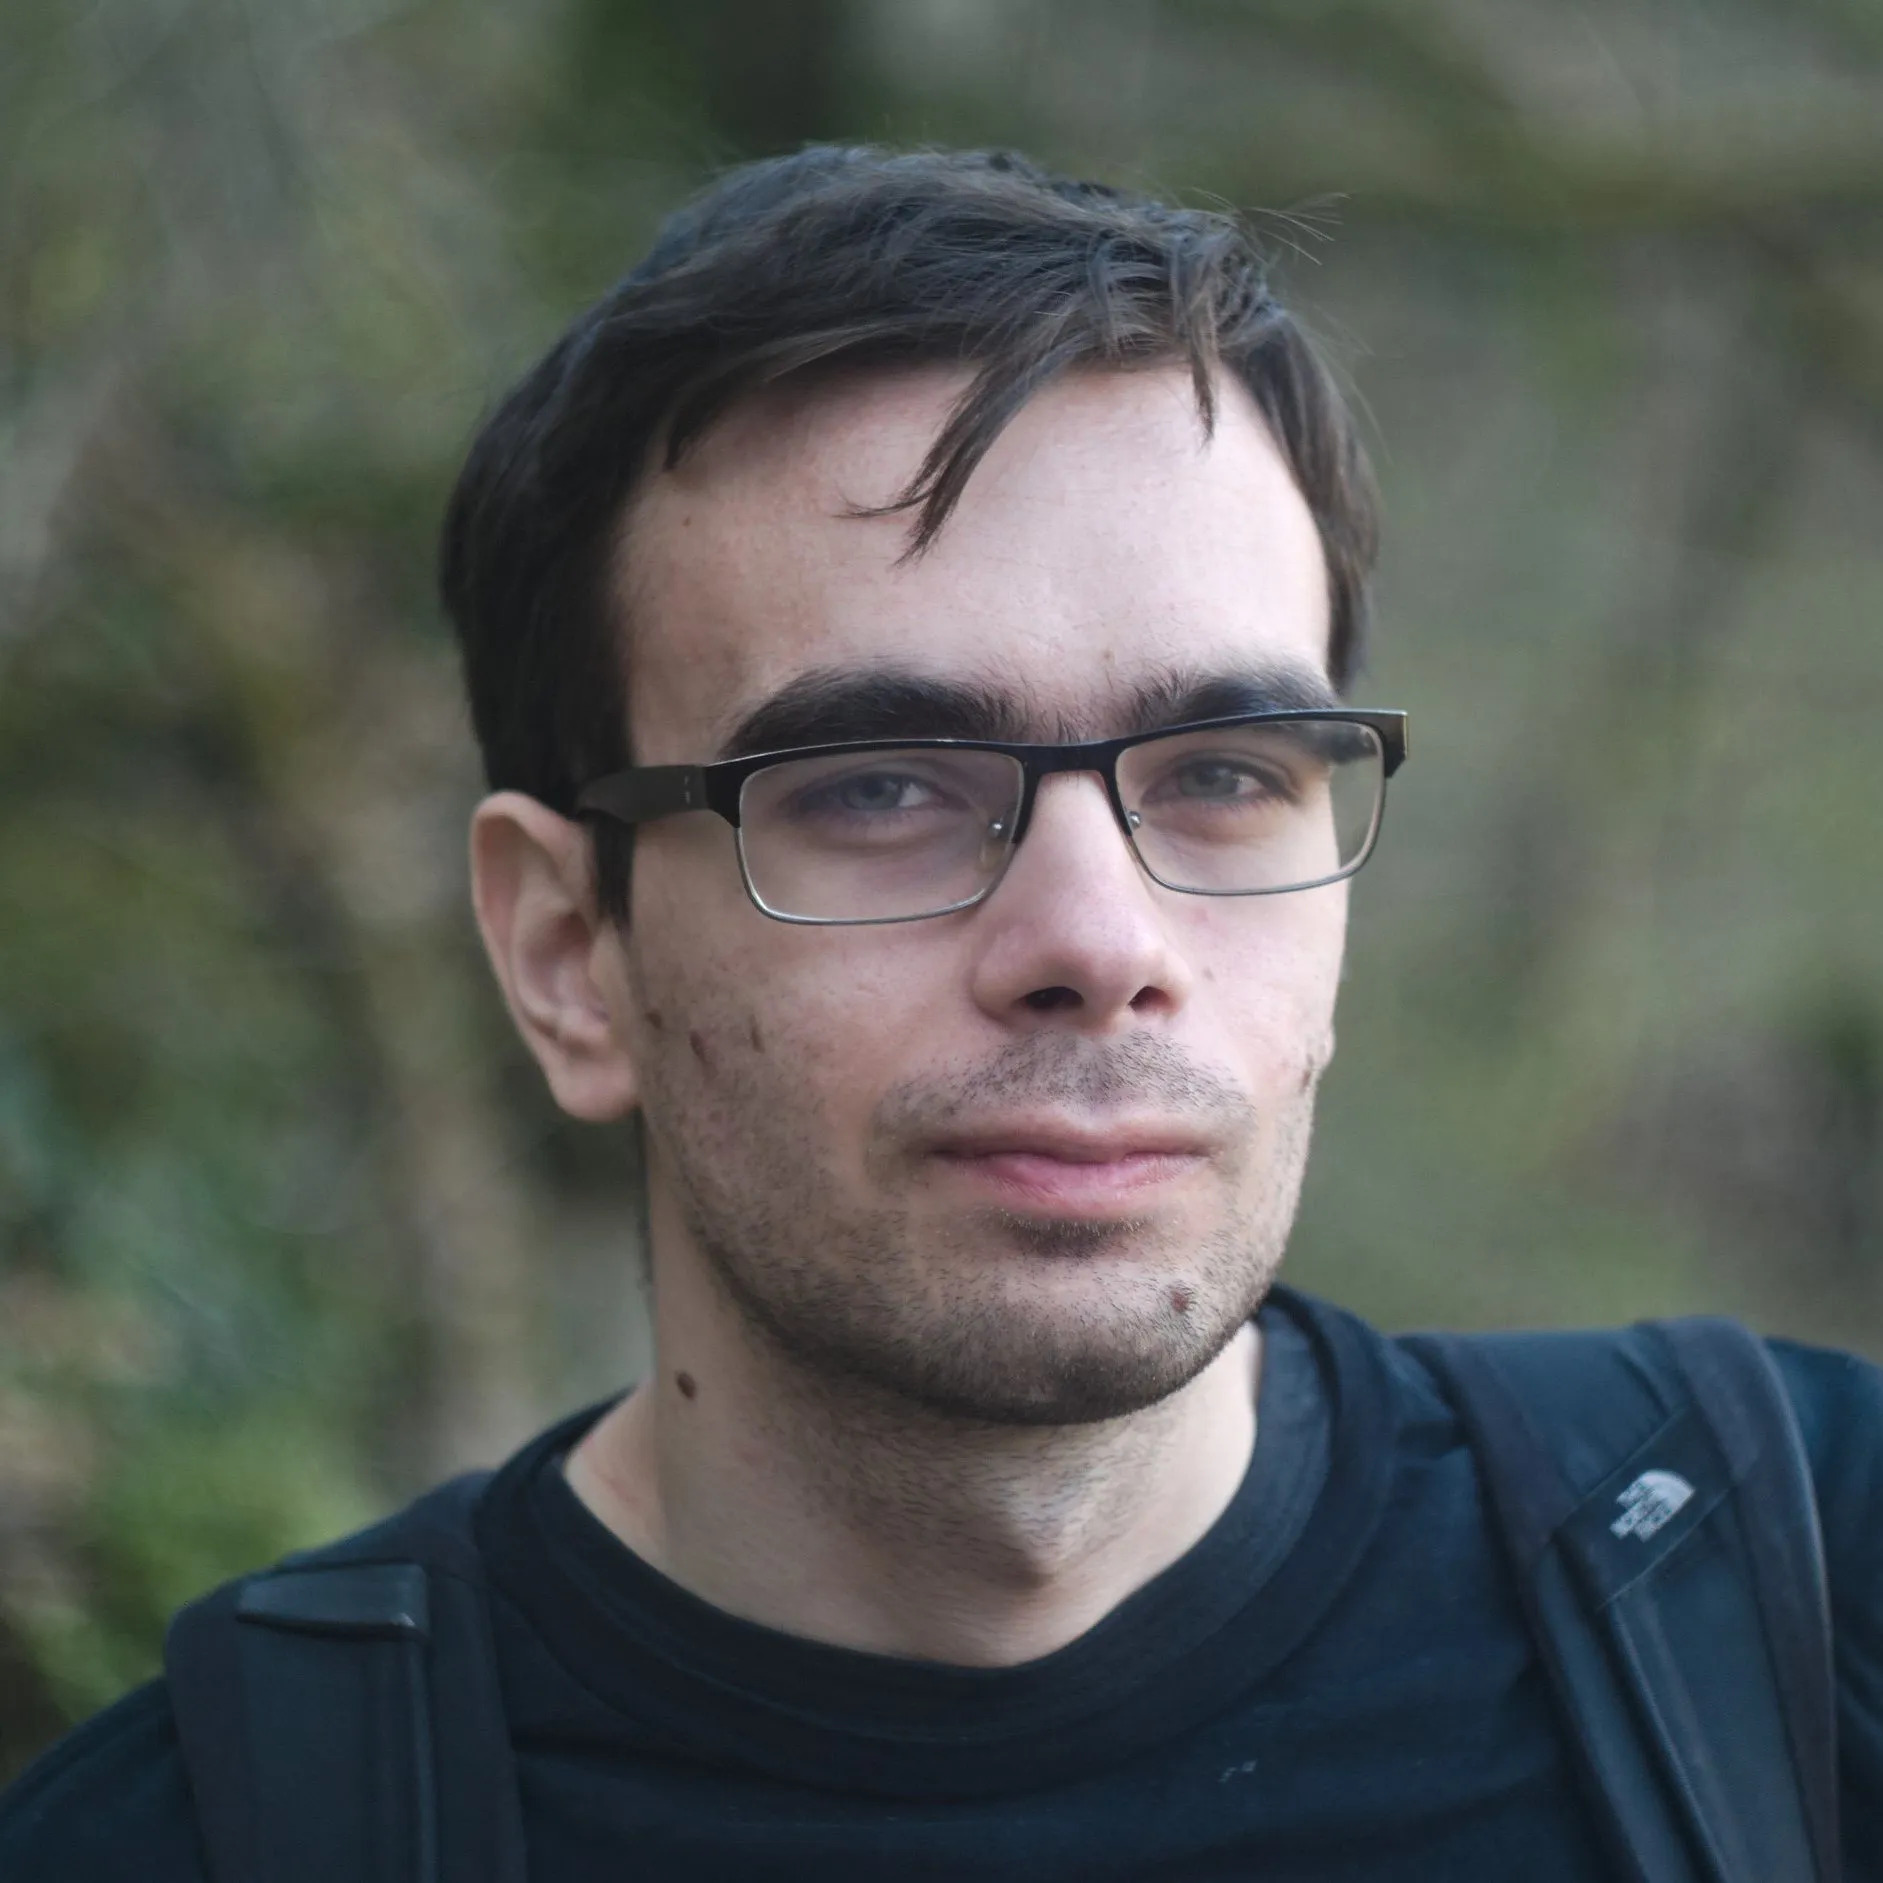
\includegraphics[width=1in,height=1.25in,clip,keepaspectratio]{media/kostas.jpg}}]{Konstantinos Kanavouras}
	is a doctoral researcher in the Space Systems Engineering research group at the University of Luxembourg's Interdisciplinary Center for Security, Reliability, and Trust (SnT). His research focuses on Systems Engineering for sub-CubeSat spacecraft, including PocketQubes and ChipSats. He has participated as an avionics and systems engineer in the AcubeSAT nanosatellite project, which is part of ESA Education’s Fly Your Satellite! programme, and has been part of the development teams of three sub-CubeSat projects in the University of Luxembourg. He received his Master's degree from the Aristotle University of Thessaloniki (Greece) in 2021.
\end{IEEEbiography}

\begin{IEEEbiography}[{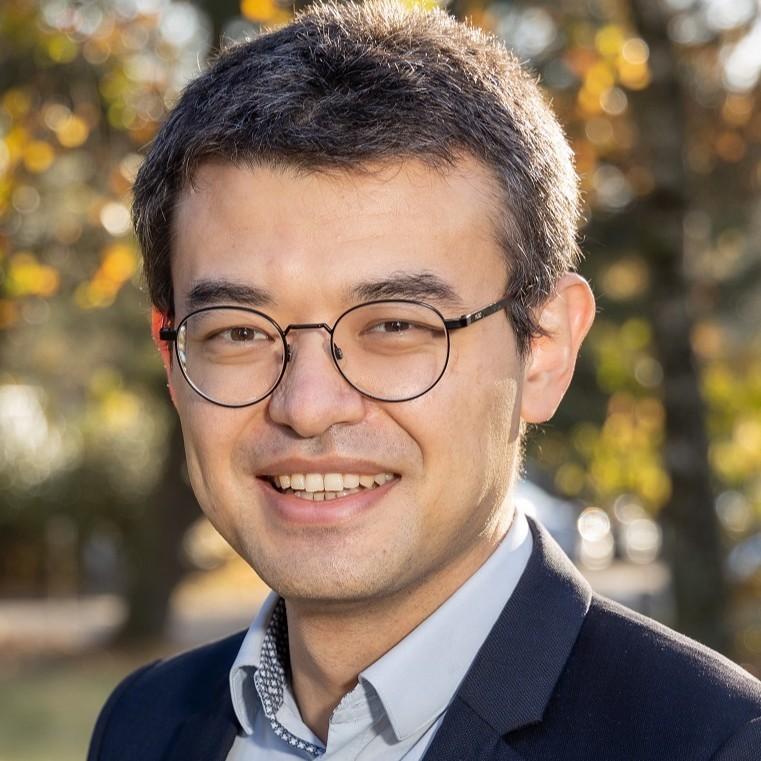
\includegraphics[width=1in,height=1.25in,clip,keepaspectratio]{media/andreas.jpg}}]{Andreas M.\ Hein}
	is an associate professor of space systems engineering at the University of Luxembourg's Interdisciplinary Center for Security, Reliability, and Trust (SnT). He works on space systems that are miniaturised and distributed, including ChipSats and CubeSats, operated in swarms and formations, in-space manufacturing, and in-situ resource utilisation. He obtained his Bachelor's and Master's degree in aerospace engineering from the Technical University of Munich and conducted his PhD research on space systems engineering there and at MIT. He has published over 70 articles in peer-reviewed international journals and conferences. For his research, Andreas has received the Exemplary Systems Engineering Doctoral Dissertation Award and the Willy Messerschmitt Award.
\end{IEEEbiography}


%\clearpage
%\newpage

\end{document}